% ──────────────────────────────────────────────────────────────────
%  NeSy-Mamba: Slot-Gated State Space Models for Interpretable
%  Logical Reasoning
%  IEEE Conference Format
% ──────────────────────────────────────────────────────────────────
\documentclass[conference]{IEEEtran}

% ── Packages ──────────────────────────────────────────────────────
\usepackage{amsmath,amssymb,amsfonts}
\usepackage{algorithmic}
\usepackage{algorithm}
\usepackage{graphicx}
\usepackage{textcomp}
\usepackage{xcolor}
\usepackage{booktabs}
\usepackage{multirow}
\usepackage{hyperref}
\usepackage{enumitem}
\usepackage{float}
\usepackage{tikz}
\usepackage{pgfplots}
\pgfplotsset{compat=newest}
\usepgfplotslibrary{groupplots}
\usetikzlibrary{positioning, arrows.meta, fit, calc, decorations.pathreplacing}

\definecolor{mamba}{RGB}{52,101,164}
\definecolor{slot}{RGB}{204,102,0}
\definecolor{lossred}{RGB}{164,0,0}
\definecolor{embed}{RGB}{78,154,6}
\definecolor{headpurp}{RGB}{117,80,123}
\definecolor{mono}{RGB}{204,0,0}
\definecolor{ema_unsup}{RGB}{52,101,164}
\definecolor{ema_sup}{RGB}{78,154,6}

% ── Macros ────────────────────────────────────────────────────────
\DeclareRobustCommand{\model}{NeSy-Mamba}
\newcommand{\Real}{\mathbb{R}}
\newcommand{\sigmoid}{\sigma}
\newcommand{\softmax}{\mathrm{softmax}}
\newcommand{\ie}{\textit{i.e.}}
\newcommand{\eg}{\textit{e.g.}}
\newcommand{\cf}{\textit{cf.}}
\newcommand{\etal}{\textit{et~al.}}
\newcommand{\wrt}{w.r.t.}

% Draft helpers (no-ops for camera-ready; restore for review)
\newcommand{\todo}[1]{}
\newcommand{\placeholder}[1]{}

\begin{document}

% ══════════════════════════════════════════════════════════════════
\title{NeSy-Mamba: Slot-Gated State Space Models\\for Interpretable Logical Reasoning}

\author{
    \IEEEauthorblockN{Samarth Bhalerao}
    \IEEEauthorblockA{
        \textit{Dept.\ of Electronics and Telecommunication} \\
        \textit{Vishwakarma Institute of Information Technology} \\
        Pune, India \\
        samarth.22211024@viit.ac.in
    }
}

\maketitle

% ══════════════════════════════════════════════════════════════════
\begin{abstract}
We introduce \model{}, a neuro-symbolic architecture that augments
selective state space models (Mamba) with a symbolic slot-gating
mechanism for interpretable multi-hop logical reasoning. While
Transformers dominate neural theorem proving, their quadratic
attention cost limits scalability, and their reasoning traces
remain opaque.  \model{} replaces attention with Mamba's
linear-time selective scan while providing built-in
interpretability through~$K$ symbolic truth-flag slots that track
the activation status of logical rules across the input sequence.

We propose an \emph{exponential moving average (EMA) slot gate}
with input-dependent memory coefficients, enabling each slot
to function as a learnable symbolic filter.  To provide
meaningful supervision, we develop a \emph{rule-type taxonomy}
that classifies ProofWriter rules into seven semantic categories
(propositional implication, propositional conjunction, relational
chaining, etc.) extracted from proof provenance, producing
structured multi-hot slot labels for training.

On the ProofWriter benchmark (118K examples, depths 0--5),
\model{} with type-based slot supervision achieves
$80.3 \pm 0.4\%$ validation accuracy (mean $\pm$ std across
seeds) with only 273K parameters.  Multi-seed evaluation
(3 seeds $\times$ 4 configurations) reveals that type-based
symbolic supervision acts as a powerful \emph{training
stabiliser}: without supervision, accuracy varies by
$\pm 6.3$--$6.6$ percentage points across seeds, whereas
type-based supervision reduces this to $\pm 0.4$~pp---a
$16\times$ reduction in variance.  While this falls short of
Transformer-based approaches such as RuleTaker ($\sim$99\%,
125M parameters)~\cite{clark2020ruletaker}, our contribution
is \emph{architectural}: demonstrating that structured state
space models can perform logical reasoning with built-in
interpretability and training stability at linear
computational cost and two orders of magnitude fewer
parameters.
We release all code and trained checkpoints.
\end{abstract}

\begin{IEEEkeywords}
neuro-symbolic AI, state space models, Mamba, interpretable
reasoning, logical inference, slot-gated networks
\end{IEEEkeywords}

% ══════════════════════════════════════════════════════════════════
\section{Introduction}
\label{sec:intro}

Multi-hop logical reasoning---the ability to chain multiple
inference steps to derive a conclusion from premises---is a
fundamental capability for trustworthy AI systems.  Given a
knowledge base of facts and rules, a reasoning engine must
determine whether a query follows logically, potentially through
several intermediate deductions.  Consider a simple example: from
the fact ``The cat is blue'' and the rule ``If something is blue
then it is kind,'' a system must deduce ``The cat is kind.''
When the proof involves two or more such steps---\emph{multi-hop}
reasoning---the task demands that the model maintain intermediate
conclusions and compose them correctly, a hallmark of systematic
generalisation~\cite{clark2020ruletaker}.

Classical symbolic systems such as Prolog backtracking engines and
answer set solvers handle this natively: they enumerate inference
paths by unification and resolution, guaranteeing soundness and
completeness within their formal scope.  However, these systems
are brittle with respect to natural language variation and cannot
learn from data---any lexical paraphrase or ambiguity breaks
resolution.  Conversely, large neural language models achieve
strong accuracy on reasoning benchmarks but operate as black
boxes, providing no insight into \emph{which rules were applied}
or \emph{in what order}~\cite{tafjord2021proofwriter}.

This tension between symbolic precision and neural flexibility
has given rise to the field of \emph{neuro-symbolic AI}, which
seeks to combine the best of both worlds.  Existing approaches
span a broad spectrum: probabilistic logic networks
(DeepProbLog~\cite{manhaeve2018deepproblog}), differentiable rule
grounding (Logic Tensor Networks~\cite{badreddine2022ltn}),
concept bottleneck models~\cite{koh2020cbm}, and retrieval-augmented
LLM pipelines~\cite{kazemi2023lambada}.  While these methods have
advanced the state of the art, they all rely on Transformer-based
backbones that incur $O(L^2)$ attention cost and provide
interpretability only through auxiliary decoders, not through the
core architecture itself.

\subsection{The Interpretability Gap}

Recent work on neural theorem provers~\cite{clark2020proofwriter,
tafjord2021proofwriter} shows that fine-tuned Transformers can
answer binary entailment queries with accuracy exceeding 95\%.
RuleTaker~\cite{clark2020ruletaker} achieves $\sim$99\% on the
ProofWriter benchmark by fine-tuning RoBERTa-large (125M
parameters).  PRover~\cite{saha2020prover} adds proof graph
generation at similar accuracy.  Despite this impressive
performance, the internal reasoning steps of these models remain
opaque.  Post-hoc explanation methods---attention
visualisation~\cite{jain2019attention}, LIME, SHAP, and
integrated gradients~\cite{sundararajan2017ig}---provide only
approximate and often unreliable attributions that do not
correspond to the actual computation performed by the model.

A model that is \emph{self-explaining by construction}---one
whose architecture explicitly represents which rules fired and
when---would offer a far stronger interpretability guarantee.
Such a model would not require post-hoc probes; instead, its
internal state would directly encode a structured representation
of the reasoning process, amenable to human inspection, formal
verification, and downstream symbolic reasoning.

\subsection{The Efficiency Gap}

Transformer-based reasoning models incur $O(L^2)$ cost in
sequence length~$L$ due to the self-attention mechanism.  For
ProofWriter theories with dozens of facts and rules, the average
sequence length is 63.4 tokens, making the quadratic cost
manageable.  However, scaling to real-world knowledge bases with
hundreds or thousands of facts would require $O(L^2)$ computation
that grows impractically.

State space models (SSMs), particularly Mamba~\cite{gu2023mamba},
offer $O(L)$ processing via selective state space recurrence.
Mamba's key innovation is \emph{input-dependent} discretisation
of the continuous-time SSM parameters ($\Delta_t, B_t, C_t$),
allowing the model to selectively attend to or ignore tokens based
on content.  This selectivity---analogous to a content-based gate
in recurrent networks---enables Mamba to match Transformer-level
performance on language modelling while maintaining linear-time
inference.  Yet despite these attractive properties, the
application of SSMs to \emph{structured logical reasoning} has not
been explored.  We hypothesise that Mamba's selective scan provides
a natural substrate for tracking which logical rules are activated
as the model processes a theory, provided an appropriate symbolic
interface is added on top.

\subsection{Our Approach}

We propose \model{}, which addresses both the interpretability and
efficiency gaps simultaneously.  The architecture consists of
three tightly integrated components:
\begin{enumerate}[nosep]
    \item A \textbf{Mamba backbone} that processes the
          fact+rule+query sequence in linear time via selective
          state space recurrence, producing contextualised hidden
          states $\mathbf{h}(t)$ at each timestep;
    \item A \textbf{symbolic slot gate} with $K$ truth-flag slots
          that track rule activations across the sequence, producing
          a structured proof trace
          $\mathbf{s}(t) \in [0,1]^K$ that evolves over the
          input---a ``soft proof trajectory'' that shows when each
          rule type becomes active;
    \item \textbf{Differentiable logic losses} that supervise the
          slots with ground-truth rule labels extracted from proof
          provenance, enforce logical implication constraints
          (answer consistency), and prevent representational
          collapse via orthogonality and entropy regularisers.
\end{enumerate}

A key technical contribution is the \emph{EMA slot gate} with
\emph{dynamic, input-dependent memory coefficients}.  Prior
slot-filling architectures~\cite{bao2022slot} use a monotonic
max gate: once a slot activates, it cannot deactivate.  We show
this leads to irreversible slot collapse where all slots converge
to the same value regardless of input content
(Section~\ref{sec:analysis}).
Our EMA gate replaces this with:
\begin{equation}
    s_k(t) = \alpha_k(t) \cdot s_k(t{-}1) + (1 - \alpha_k(t)) \cdot \hat{s}_k(t)
\label{eq:ema_intro}
\end{equation}
where $\alpha_k(t) = \sigma(W_\alpha \cdot h_t + b_{\alpha_k})$
is a learned, per-token, per-slot memory coefficient.  This
formulation makes each slot a \emph{GRU-like symbolic filter}:
the model learns to retain evidence when it encounters supporting
tokens and to update its belief when it encounters contradicting
evidence.  The dynamic nature of $\alpha_k(t)$---computed as a
function of the current hidden state---means that the same slot
can behave differently at different positions in the sequence,
enabling fine-grained temporal tracking of rule activations.

\subsection{Key Finding: Supervision as Stabilisation}

Perhaps our most surprising finding is that symbolic supervision
serves not merely as an interpretability mechanism, but as a
\emph{training stabiliser}.  Multi-seed evaluation (3~seeds
$\times$ 4~configurations) reveals that without type-based
supervision, accuracy varies by $\pm 6.3$--$6.6$ percentage
points across seeds---a range that encompasses both the best
(80.6\%) and worst (65.3\%) results.  With type-based
supervision ($\lambda_s{=}1.0$), this variance collapses to
$\pm 0.4$~pp, a $16\times$ reduction.  This finding has
practical implications for small-model training: structured
symbolic supervision provides the inductive bias needed to
escape poor local minima that plague low-capacity models.

\subsection{Contributions}

\begin{enumerate}[nosep]
    \item We introduce \model{}, the first architecture combining
          selective SSMs with symbolic slot-gating for logical
          reasoning, demonstrating that SSMs can perform
          non-trivial multi-hop inference with built-in
          interpretability at linear computational cost.
    \item We identify the \emph{monotonic slot collapse} problem
          in max-gated neuro-symbolic architectures and propose
          the EMA gate with dynamic~$\alpha$ as a principled
          alternative, grounded in the formal connection between
          exponential moving average dynamics and GRU update gates.
    \item We develop a \emph{rule-type taxonomy} that classifies
          ProofWriter rules into seven semantic categories from
          proof provenance, enabling supervised slot assignment
          with structured multi-hot labels.
    \item Through multi-seed ablation (3 seeds $\times$ 4
          configurations) we demonstrate that type-based symbolic
          supervision reduces cross-seed accuracy variance by
          $16\times$ ($\pm 0.4\%$ vs.\ $\pm 6.3$--$6.6\%$),
          establishing supervised slot assignment as a training
          stabiliser, not merely an interpretability aid.
    \item We release all code, training logs, and multi-seed
          results for full reproducibility.
\end{enumerate}

The remainder of this paper is organised as follows.
Section~\ref{sec:related} reviews related work.
Section~\ref{sec:method} describes the \model{} architecture
in detail.  Section~\ref{sec:experiments} presents the
experimental setup.  Section~\ref{sec:results} reports results.
Section~\ref{sec:analysis} provides detailed analysis of slot
dynamics and the collapse problem.
Section~\ref{sec:discussion} discusses implications and
limitations, and Section~\ref{sec:conclusion} concludes.


% ══════════════════════════════════════════════════════════════════
\section{Related Work}
\label{sec:related}

\subsection{State Space Models for Sequence Modelling}

Structured state space models (S4)~\cite{gu2022s4} demonstrated
that linear recurrences with structured initialisation (HiPPO
matrices) can match or exceed Transformers on long-range
benchmarks such as the Long Range Arena.  The key insight is that
continuous-time state space equations, when discretised with
appropriate step sizes, capture long-range dependencies that RNNs
and LSTMs famously struggle with.  S4 parameterises the state
matrix as a low-rank plus diagonal structure, enabling efficient
training via FFT-based convolution.

Mamba~\cite{gu2023mamba} extended this paradigm with
\emph{selective} state transitions---making the SSM parameters
($\Delta$, $B$, $C$) input-dependent functions of the current
token.  This selectivity allows the model to dynamically decide
how much to store or discard at each timestep, providing a
content-based gating mechanism analogous to attention but at
$O(L)$ cost.  The hardware-aware selective scan algorithm enables
efficient GPU implementation.  Mamba achieves Transformer-level
language modelling quality with linear-time inference and has been
adopted across multiple domains: Vim~\cite{zhu2024vim} for vision
(bidirectional state space scanning of image patches),
genomics~\cite{gu2023mamba} for DNA sequence modelling, and time
series forecasting.

Subsequent work has introduced Mamba-2 with improved
parallelisation via structured masked attention duality, and
hybrid architectures that combine Mamba layers with sparse
attention for tasks requiring explicit long-range token
interaction.  However, the application of Mamba or any SSM variant
to \emph{structured symbolic reasoning}---where the model must
track logical rule activations and compose multi-step
inferences---remains entirely unexplored.  \model{} fills this gap
by augmenting Mamba's efficient sequential processing with explicit
symbolic slots that transform the SSM's hidden state dynamics into
interpretable rule-tracking signals.

\subsection{Neural Theorem Proving}

The ProofWriter benchmark~\cite{tafjord2021proofwriter} frames
logical reasoning as binary classification: given a theory (facts
+ rules) and a query, predict whether the query is entailed.
The dataset spans proof depths 0--5, with depth-0 requiring simple
fact lookup and depth-5 requiring five chained inference steps.
This controlled setting enables precise evaluation of reasoning
capability as a function of compositional depth.

RuleTaker~\cite{clark2020ruletaker} established the dominant
approach: fine-tuning RoBERTa-large (125M parameters) on
theory+query pairs achieves $\sim$99\% accuracy.  The model
successfully generalises across proof depths, though it provides
no insight into the reasoning path.
PRover~\cite{saha2020prover} extends RuleTaker by jointly
predicting proof graphs alongside answers, achieving $\sim$95\%
answer accuracy and providing interpretable proof traces.  However,
the proof generation is handled by an \emph{auxiliary} decoder, not
by the core prediction architecture itself.

LAMBADA~\cite{kazemi2023lambada} takes a different approach, using
backward chaining with large language models (LLMs) to decompose
queries into sub-goals and recursively verify them against the
knowledge base.  This provides more natural reasoning traces but
incurs the $O(L^2)$ cost of Transformer attention at each step,
compounded by multiple inference passes for backward chaining.

Other related work includes chain-of-thought prompting for
reasoning~\cite{wei2022chain}, which elicits step-by-step
reasoning from LLMs but without formal guarantees of logical
soundness.  Selection-inference~\cite{creswell2022selection}
decomposes reasoning into alternating selection and inference
modules, improving compositional generalisation.

All these approaches share two common characteristics: (i)~they
rely on Transformer backbones with $O(L^2)$ attention cost, and
(ii)~interpretability is provided only through auxiliary outputs
(proof decoders, chain-of-thought text, attention maps), not
through the core architecture itself.  \model{} does not aim to
match these accuracy levels---our 273K-parameter model operates
at a fundamentally different scale than 125M-parameter
RoBERTa.  Instead, we explore whether structured SSMs can serve
as efficient, self-explaining reasoning backbones where
interpretability is built into the hidden state via symbolic
slot gates.

\subsection{Neuro-Symbolic Integration}

Neuro-symbolic methods combine neural perception with symbolic
reasoning, spanning a broad spectrum of integration depth:

\textbf{Logic programming integration.}
DeepProbLog~\cite{manhaeve2018deepproblog} integrates neural
networks with probabilistic logic programming, allowing neural
outputs to serve as probabilistic facts in ProbLog programs.
NeurASP~\cite{yang2020neurasp} combines neural networks with
answer set programming, enabling learned perception to feed
symbolic constraint satisfaction.  These methods provide strong
logical guarantees but require explicit symbolic programs and
struggle with end-to-end differentiability.

\textbf{Differentiable logic.}
Logic Tensor Networks~\cite{badreddine2022ltn} ground
first-order logic formulas in differentiable tensor operations,
enabling end-to-end training with logical constraints as
regularisers.  This approach is closest to our differentiable
logic losses, but operates on object-level features rather than
sequential rule activations.

\textbf{Concept bottleneck architectures.}
Concept Bottleneck Models~\cite{koh2020cbm} route predictions
through interpretable concept layers, forcing the model to
represent human-understandable intermediate features.  Our slot
gate is conceptually related---each slot represents a
human-interpretable concept (rule type)---but operates in a
sequential, temporal setting where slot values evolve over the
input sequence rather than being computed in a single forward
pass.

\textbf{Slot-structured representations.}
Slot Attention~\cite{locatello2020slot} learns object-centric
representations via iterative attention over a set of slot vectors.
Object-centric models decompose scenes into discrete object
representations, enabling compositional generalisation.  Our work
is related in spirit but differs fundamentally: our slots represent
\emph{truth values of logical rules} rather than object features,
and we use \emph{recurrent SSM processing} rather than iterative
attention for slot updates.

Our work occupies a unique position in this landscape: we combine
the sequential efficiency of SSMs with explicit symbolic slots
supervised by differentiable logic constraints.  The three key
differentiators of our approach are: (i)~recurrent SSM backbone
instead of attention, (ii)~slots as truth-flag values rather than
object features, and (iii)~temporal EMA dynamics that provide
\emph{when} during the sequence each rule was applied---a
capability absent from all prior neuro-symbolic architectures.

\subsection{Gating Mechanisms and Temporal Dynamics}

The EMA slot gate draws on a rich history of gating mechanisms
in recurrent networks.

\textbf{GRU and LSTM gates.}
GRUs~\cite{cho2014gru} use update and reset gates to control
information flow through hidden states.  Our dynamic $\alpha_k(t)$
is functionally analogous to the GRU update gate
$z_t = \sigma(W_z x_t + U_z h_{t-1})$, but applied to
\emph{symbolic truth-flag slots} rather than dense hidden states.
The key difference is that our slots are \emph{interpretable by
design}: each $s_k(t)$ has a semantic label (rule type), and the
$\alpha_k(t)$ trajectory reveals the temporal dynamics of that
rule's activation.

\textbf{Monotonic and irreversible gates.}
The monotonic max gate we replace is similar to the CumMax
mechanism in Ordered Neurons (ON-LSTM~\cite{shen2019ordered}),
where an irreversible accumulation enforces a hierarchical
grouping of information.  While ON-LSTM's irreversibility is
desirable for modelling syntactic structure (higher-level
constituents should persist longer), we show that irreversibility
is \emph{harmful} for slot differentiation in the reasoning
setting: once all slots ratchet to the same value, they carry
zero information about the specific logical rules applied in each
example (Section~\ref{sec:analysis}).

\textbf{Exponential moving averages in deep learning.}
EMA appears throughout deep learning: in batch normalisation
(running statistics), in target network updates
(DQN, BYOL), and in recent work on EMA-based attention
mechanisms.  Our use of EMA is distinctive in that the smoothing
coefficient $\alpha_k(t)$ is itself learned and input-dependent,
making it an adaptive temporal filter rather than a fixed
smoothing operator.  This adaptivity is essential for reasoning:
the same slot should have high $\alpha$ (strong memory) when
processing irrelevant tokens and low $\alpha$ (rapid update) when
encountering evidence for or against its associated rule.


% ══════════════════════════════════════════════════════════════════
\section{Method}
\label{sec:method}

\model{} combines three modules: a Mamba backbone for sequence
encoding (Section~\ref{sec:backbone}), a symbolic slot gate for
rule tracking (Section~\ref{sec:slotgate}), and differentiable
logic losses for structured supervision
(Section~\ref{sec:logicloss}).  The full architecture is
illustrated in Figure~\ref{fig:architecture}.

\begin{figure}[t]
    \centering
    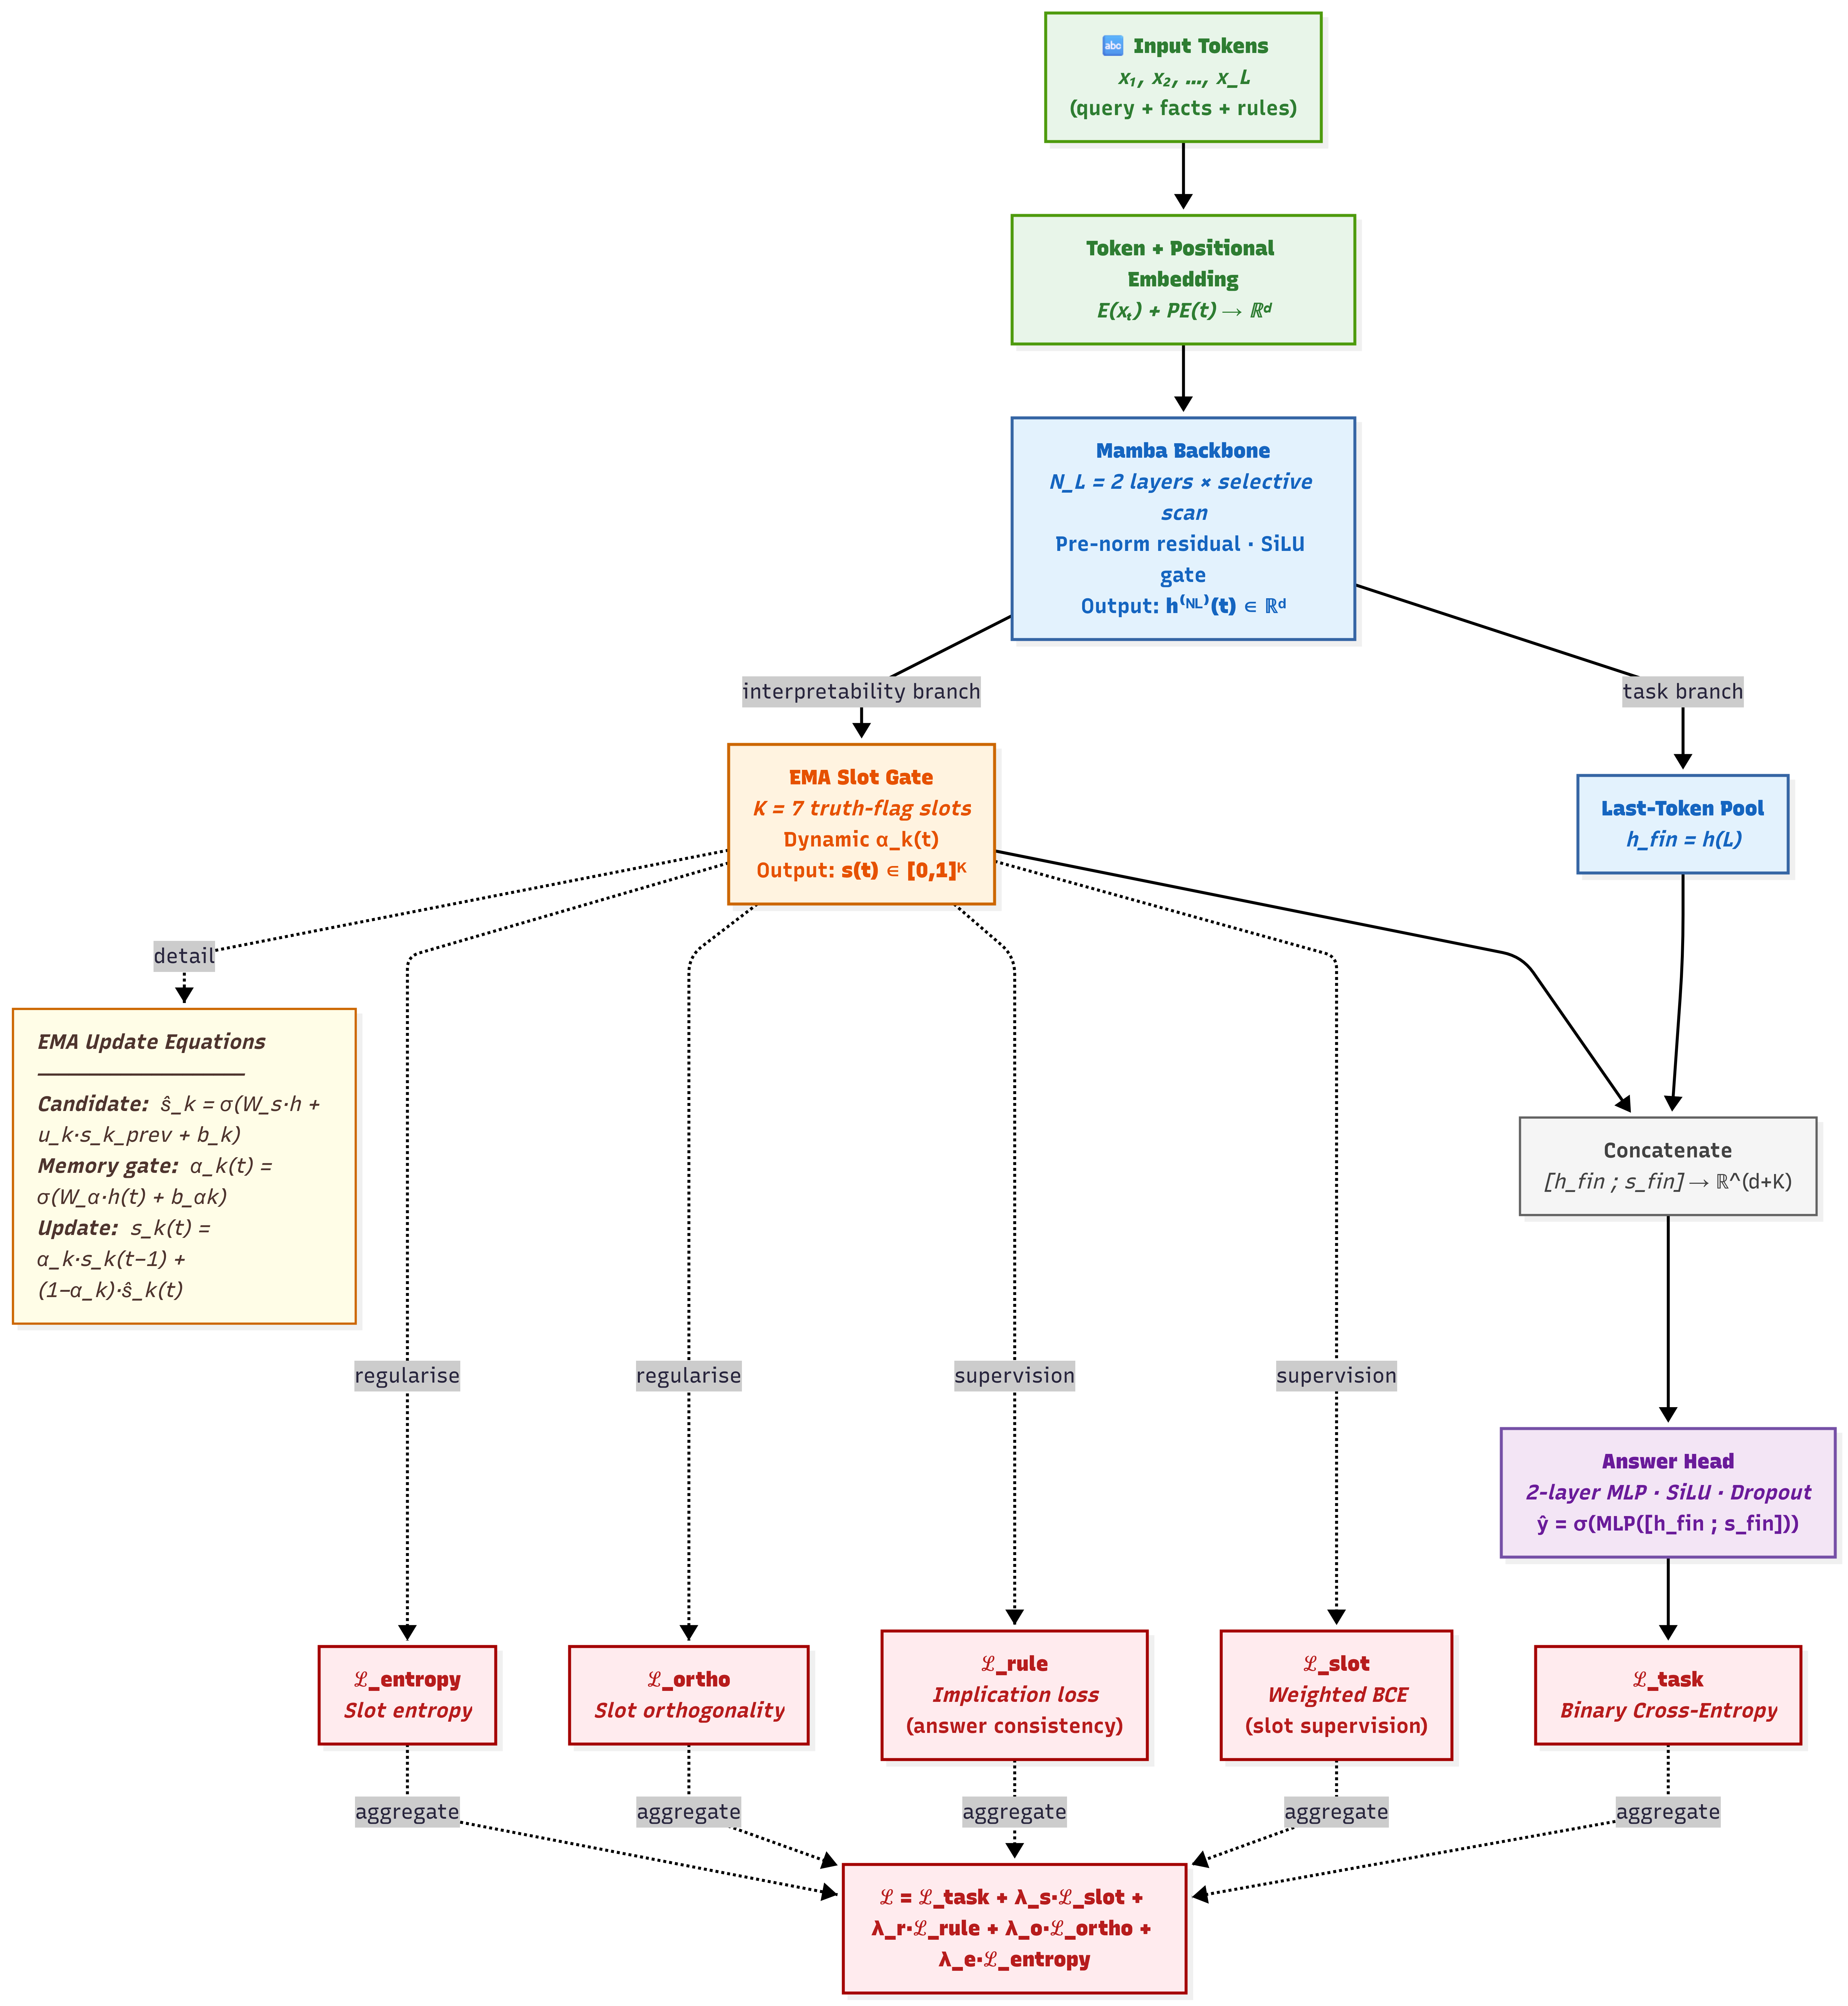
\includegraphics[width=\columnwidth]{architecture.png}
    \caption{\textbf{Architecture of \model{}.}  The Mamba backbone
    processes the tokenised theory+query in $O(L)$ time via
    selective scan.  Hidden states $\mathbf{h}(t)$ feed two branches:
    (i)~last-token pooling for the answer head, and (ii)~the EMA
    slot gate, which maintains $K{=}7$ symbolic truth-flag
    values $\mathbf{s}(t) \in [0,1]^K$.  The input-dependent memory
    coefficient $\alpha_k(t)$ allows each slot to selectively retain
    or update its belief at every timestep.  Five differentiable
    losses jointly train the system: task BCE, slot supervision,
    answer consistency, orthogonality, and entropy regularisation.
    Dashed arrows indicate supervision signals; solid arrows
    indicate data flow.}
    \label{fig:architecture}
\end{figure}

At a high level, the forward pass proceeds as follows: (i)~tokenise
the concatenated query+facts+rules string and embed each token;
(ii)~pass the embedded sequence through $N_L$ Mamba blocks to
obtain contextualised hidden states; (iii)~update $K$ slot values
at each timestep via the EMA gate; (iv)~concatenate the final
hidden state with the final slot vector and predict the answer
through a two-layer MLP.  During training, four differentiable
losses are applied to the slot activations in addition to the
task loss.  Algorithm~\ref{alg:forward} formalises this.

\begin{algorithm}[t]
\caption{\model{} Forward Pass and Loss Computation}
\label{alg:forward}
\begin{algorithmic}[1]
\REQUIRE Theory+query sequence $x = (x_1, \ldots, x_L)$,
  slot labels $\mathbf{s}^* \in \{0,1\}^K$ (if supervised),
  answer label $y^*$
\STATE \textbf{Embed:} $\mathbf{e}(t) \leftarrow \mathrm{Emb}(x_t) + \mathrm{Pos}(t)$
        for $t = 1, \ldots, L$
\STATE \textbf{Mamba:} $\mathbf{h}^{(0)}(t) \leftarrow \mathbf{e}(t)$
\FOR{$l = 1$ to $N_L$}
    \STATE $\mathbf{h}^{(l)} \!\leftarrow\! \mathbf{h}^{(l-1)} \!+\!
        \mathrm{Drop}(\mathrm{Mamba}^{(l)}(\mathrm{RMSNorm}(\mathbf{h}^{(l-1)})))$
\ENDFOR
\STATE \textbf{Slot Gate:} Initialise $\mathbf{s}(0) \leftarrow \mathbf{0}$
\FOR{$t = 1$ to $L$}
    \STATE $\hat{s}_k(t) \leftarrow \sigma(W_s \mathbf{h}^{(N_L)}(t) + u_k s_k(t{-}1) + b_k)$ for each $k$
    \STATE $\alpha_k(t) \leftarrow \sigma(W_\alpha \mathbf{h}^{(N_L)}(t) + b_{\alpha_k})$
    \STATE $s_k(t) \leftarrow \alpha_k(t) \cdot s_k(t{-}1) + (1-\alpha_k(t)) \cdot \hat{s}_k(t)$
\ENDFOR
\STATE \textbf{Pool:} $\mathbf{h}_{\mathrm{fin}} \leftarrow \mathbf{h}^{(N_L)}[\ell-1]$ \COMMENT{last real token}
\STATE \textbf{Predict:} $\hat{y} \leftarrow \sigma(\mathrm{MLP}([\mathbf{h}_{\mathrm{fin}}; \mathbf{s}(L)]))$
\STATE \textbf{Losses:}
\STATE $\quad \mathcal{L}_{\text{task}} \leftarrow \mathrm{BCE}(\hat{y}, y^*)$
\STATE $\quad \mathcal{L}_{\text{slot}} \leftarrow \text{WeightedBCE}(\mathbf{s}(L), \mathbf{s}^*)$
\STATE $\quad \mathcal{L}_{\text{rule}} \leftarrow \text{AnswerConsistency}(\mathbf{s}(L), \hat{y})$
\STATE $\quad \mathcal{L}_{\text{ortho}} \leftarrow \|{\hat{S}^\top \hat{S} - I_K}\|_F$
\STATE $\quad \mathcal{L}_{\text{entropy}} \leftarrow \text{SlotEntropy}(\mathbf{s})$
\STATE $\quad \mathcal{L} \leftarrow \mathcal{L}_{\text{task}} + \lambda_s \mathcal{L}_{\text{slot}} + \lambda_r \mathcal{L}_{\text{rule}} + \lambda_o \mathcal{L}_{\text{ortho}} + \lambda_e \mathcal{L}_{\text{entropy}}$
\RETURN $\hat{y}$, $\mathbf{s}(1), \ldots, \mathbf{s}(L)$, $\mathcal{L}$
\end{algorithmic}
\end{algorithm}

\subsection{Input Representation}
\label{sec:input}

Each input consists of a theory $\\mathcal{T} = \\{f_1, \\dots, f_M,
r_1, \\dots, r_N\\}$ of facts and rules expressed in natural
language, together with a query~$q$.  These are concatenated into
a single input sequence $x$:
\begin{equation}
    x = [q\ ;\ f_1\ ;\ \dots\ ;\ f_M\ ;\ r_1\ ;\ \dots\ ;\ r_N]
\end{equation}
The query is placed first so that the Mamba backbone can condition
its selective scan on the information need before processing the
theory---analogous to the ``question-first'' ordering used in
reading comprehension models.  Structural separator tokens
(\texttt{[FACT]}, \texttt{[RULE]}, \texttt{[SEP]}) are inserted
between segments to provide explicit boundary signals.

Tokenisation uses a punctuation-aware splitter that segments on
whitespace and punctuation marks, producing a vocabulary of 41
unique tokens for ProofWriter.  This compact vocabulary reflects
the controlled language of the benchmark (entities like ``cat,''
``dog''; properties like ``blue,'' ``kind''; and logical
connectives like ``if,'' ``then,'' ``and'').

Token and learned positional embeddings are summed:
$\mathbf{e}(t) = \mathrm{Emb}(x_t) + \mathrm{Pos}(t)$,
followed by dropout ($p = 0.1$).  The positional embeddings are
learned (not sinusoidal), initialised from $\mathcal{N}(0, 0.02)$,
with a maximum length of 256 tokens (sufficient for all
ProofWriter examples, whose maximum length is 194 tokens).

\textbf{Padding and masking.}  Variable-length sequences within
a batch are right-padded to the maximum length, and a binary
mask $\mathbf{m} \in \{0,1\}^{L_{\max}}$ is maintained.  The
Mamba scan ignores padded positions via masking in the output
projection, and the last-token pooling indexes the final
non-padded position per example.

\subsection{Mamba Backbone}
\label{sec:backbone}

The embedded sequence is processed by a stack of $N_L = 2$ Mamba
blocks with pre-norm residual connections:
\begin{equation}
    \mathbf{h}^{(l)} = \mathbf{h}^{(l-1)} +
    \mathrm{Dropout}\!\left(\mathrm{Mamba}\!\left(
    \mathrm{RMSNorm}(\mathbf{h}^{(l-1)})\right)\right)
\end{equation}
We use RMSNorm~\cite{zhang2019rms} rather than LayerNorm for
marginal computational savings and stable training dynamics.

\subsubsection{Internal Mamba Block Architecture}

Each Mamba block consists of four stages:
\begin{enumerate}[nosep]
    \item \textbf{Double projection:} A linear layer maps from
          $d_{\text{model}}$ to $2d_{\text{inner}}$ (expand
          factor~2, so $d_{\text{inner}} = 256$).  The output is
          split into a branch~$\mathbf{x}_B$ that enters the SSM
          pathway and a gate~$\mathbf{z}$ that modulates the output;
    \item \textbf{Causal convolution:} A depth-wise 1-D convolution
          with kernel size $d_c = 4$ and causal padding is applied
          to $\mathbf{x}_B$, followed by SiLU activation.  This
          local mixing provides a short-range inductive bias
          complementary to the SSM's long-range dynamics;
    \item \textbf{Selective state space recurrence:} The core
          computation that makes Mamba differ from prior SSMs.
          The discretisation parameters ($\Delta_t$, $B_t$, $C_t$)
          are computed as linear projections of the current token,
          making state transitions \emph{content-dependent};
    \item \textbf{Gated output:} The SSM output is element-wise
          multiplied with $\mathrm{SiLU}(\mathbf{z})$ and projected
          back to $d_{\text{model}}$:
          $\mathbf{y} = (\mathbf{y}_{\text{SSM}} \odot
          \mathrm{SiLU}(\mathbf{z})) \cdot W_{\text{out}}$.
\end{enumerate}

\subsubsection{Selective Scan Mechanism}

The selective SSM discretises continuous-time parameters into
recurrence coefficients:
\begin{align}
    \bar{A}_t &= \exp(\Delta_t \cdot A) \label{eq:disc_a} \\
    \bar{B}_t &= \Delta_t \cdot B_t \label{eq:disc_b} \\
    h_t &= \bar{A}_t \cdot h_{t-1} + \bar{B}_t \cdot x_t
    \label{eq:ssm_recurrence} \\
    y_t &= C_t \cdot h_t + D \cdot x_t \label{eq:ssm_output}
\end{align}
where $A \in \Real^{D \times N}$ is initialised in log-space
using a HiPPO-inspired scheme that promotes long-range signal
propagation.  The state dimension $N = d_{\text{state}} = 16$
provides a compact but sufficient latent representation.

The key insight of Mamba's selectivity is that $\Delta_t$ controls
\emph{how much} the current token is integrated into the state:
large $\Delta_t$ makes $\bar{A}_t \approx 0$ (forget the past,
absorb the input), while small $\Delta_t$ makes $\bar{A}_t
\approx I$ (retain the past, ignore the input).  For logical
reasoning, this selectivity is crucial: the model can learn to
``attend'' to rule-relevant tokens (``if,'' ``then,'' entity names)
while passing over filler tokens (``is,'' ``the'').

The step size $\Delta_t$ is computed via a low-rank projection:
$\Delta_t = \mathrm{softplus}(W_{\Delta} \cdot x_t + b_\Delta)$,
where $W_\Delta \in \Real^{d_{\text{inner}} \times d_\Delta}$
(rank $d_\Delta = 2$) followed by broadcast.  The softplus
ensures positivity.  The bias $b_\Delta$ is initialised via the
inverse-softplus uniform scheme of~\cite{gu2023mamba}, maintaining
stable dynamics during early training.

\subsubsection{Last-Token Pooling}

The final hidden state is obtained via last-real-token pooling:
$\mathbf{h}_{\text{final}} = \mathbf{h}^{(N_L)}[\ell_i - 1]$
where $\ell_i$ is the number of non-padding tokens in example $i$.
This strategy leverages the causal nature of the SSM: the last
token's hidden state contains information from the entire sequence,
as the recurrence propagates information forward through time.
Unlike bidirectional encoders (e.g., BERT's \texttt{[CLS]} token),
unidirectional pooling introduces an ordering dependence, which
we mitigate by placing the query first in the input sequence.

\subsection{Symbolic Slot Gate}
\label{sec:slotgate}

The slot gate maintains $K$ scalar truth-flag values
$\mathbf{s}(t) = [s_1(t), \dots, s_K(t)] \in [0,1]^K$ that are
updated at every timestep.  Each slot represents the model's
soft belief that a particular logical rule has fired.

\subsubsection{Candidate Computation}

At each timestep $t$, a candidate activation is computed for each
slot:
\begin{equation}
    \hat{s}_k(t) = \sigma\!\left(
    \underbrace{W_s \cdot \mathbf{h}(t)}_{\text{input-dependent}}
    + \underbrace{u_k \cdot s_k(t{-}1)}_{\text{recurrence}}
    + \underbrace{b_k}_{\text{bias}}
    \right)
\label{eq:candidate}
\end{equation}
where $W_s \in \Real^{K \times d}$ is a shared projection
(Xavier init with gain $g_s$), $u_k$ is a per-slot diagonal
recurrence weight, and $b_k$ is a per-slot bias. The diagonal
recurrence preserves per-slot identity for interpretability, as
opposed to a full $K \times K$ coupling matrix.

\subsubsection{Optional Slot Competition}

To encourage specialisation (one dominant slot per timestep), we
optionally apply temperature-scaled softmax competition:
\begin{equation}
    \tilde{s}_k(t) = \frac{\exp(\hat{s}_k(t) / \tau)}
    {\sum_{j=1}^K \exp(\hat{s}_j(t) / \tau)} \cdot \hat{s}_k(t)
\label{eq:competition}
\end{equation}
where $\tau$ is a temperature hyperparameter.

\subsubsection{Gate Update: Monotonic Max vs. EMA}

\textbf{Monotonic max (baseline).}
The original gate accumulates evidence irreversibly:
\begin{equation}
    s_k(t) = \max\!\left(s_k(t{-}1),\ \tilde{s}_k(t)\right)
\label{eq:monotonic}
\end{equation}
This models proof accumulation (once a fact is deduced, it
persists) but prevents the model from learning \emph{negative
evidence} and causes all slots to converge to the same value
(Section~\ref{sec:analysis}).

\textbf{EMA gate (proposed).}
We replace the monotonic max with an exponential moving average:
\begin{equation}
    s_k(t) = \alpha_k(t) \cdot s_k(t{-}1) +
    (1 - \alpha_k(t)) \cdot \tilde{s}_k(t)
\label{eq:ema}
\end{equation}
The memory coefficient $\alpha_k(t)$ controls the trade-off
between retaining the previous slot value (memory) and accepting
the new candidate (update).

\textbf{Dynamic $\alpha$ (full model).}
We make $\alpha$ input-dependent via a learned linear projection:
\begin{equation}
    \alpha_k(t) = \sigma\!\left(
    W_\alpha \cdot \mathbf{h}(t) + b_{\alpha_k}
    \right)
\label{eq:dynamic_alpha}
\end{equation}
where $W_\alpha \in \Real^{K \times d}$ is initialised with small
gain (0.1) and the biases $b_{\alpha_k}$ are stagger-initialised
around a high base value ($\sigma(2.0) \approx 0.88$) for symmetry
breaking.  This makes each slot a \emph{learnable symbolic filter}:
the model decides per-token how much each slot should retain its
current belief versus update based on new evidence.  This is
analogous to the GRU~\cite{cho2014gru} update gate, but applied
to symbolic truth-flag slots rather than dense hidden states.

\textbf{Static $\alpha$ (ablation).}
For ablation, we also implement a static variant where each slot
has a single learnable $\alpha_k = \sigma(\ell_k)$, independent
of input.  This isolates the contribution of input-dependence from
the EMA mechanism itself.

\subsubsection{Initialisation Strategy}
\label{sec:init}

The initialisation of the slot gate parameters is critical for
avoiding early collapse.  We employ the following strategy, derived
from ablation over initialisation schemes:

\begin{itemize}[nosep]
    \item \textbf{Slot projection $W_s$:} Xavier uniform with
          gain $g_s = 1.0$.  Lower gains (e.g., $g_s = 0.1$)
          suppress the input signal relative to the bias, causing
          the bias to dominate and all slots to converge to the
          same fixed point.  This was the root cause of collapse
          in early experiments (Section~\ref{sec:analysis}).
    \item \textbf{Recurrence weights $u_k$:} Initialised to
          $+0.01$ (small positive).  This provides a mild
          self-reinforcing tendency: slots that activate tend to
          remain active, modelling the ``accumulation of evidence''
          intuition.  Negative values cause oscillation; large
          positive values cause runaway activation.
    \item \textbf{Bias $b_k$:} All zeros.  Combined with
          $\sigma(0) = 0.5$, this centres the initial candidates
          around 0.5.  The EMA dynamics then push slots toward
          their learned equilibria.
    \item \textbf{Alpha projection $W_\alpha$:} Xavier uniform
          with small gain (0.1).  The small gain ensures that
          initially, $\alpha_k(t) \approx \sigma(b_{\alpha_k})$
          for all tokens, so the gate starts in a near-static
          regime and gradually learns to differentiate.
    \item \textbf{Alpha biases $b_{\alpha_k}$:} Stagger-initialised
          around a high base value.  Specifically,
          $b_{\alpha_k} = 2.0 + 0.05 \cdot k$ for
          $k \in \{0, \ldots, K{-}1\}$, giving
          $\alpha_k(0) \in [0.88, 0.89]$.  The high initial
          $\alpha$ makes slots ``sticky'' at startup (strong
          memory, slow update), preventing rapid convergence to
          degenerate fixed points.  The staggering breaks symmetry
          so that different slots start with slightly different
          temporal dynamics.
\end{itemize}

\subsubsection{Firing Order Tracking}

We track the timestep at which each slot first crosses the
activation threshold~$\theta$:
\begin{equation}
    \text{fire}_k = \min\{t : s_k(t) > \theta\}
\end{equation}
This provides a temporal ordering over rule activations---a proxy
for the proof execution trace.

\subsection{Answer Head}
\label{sec:answer}

The final prediction concatenates the Mamba output and slot values
into a joint representation:
\begin{equation}
    \hat{y} = \sigma\!\left(\mathrm{MLP}\!\left(
    [\mathbf{h}_\text{final}\ ;\ \mathbf{s}_\text{final}]
    \right)\right)
\end{equation}
The MLP consists of two fully connected layers:
\begin{align}
    \mathbf{z}_1 &= \mathrm{SiLU}\!\left(W_1 [\mathbf{h}_{\text{final}}; \mathbf{s}_{\text{final}}] + \mathbf{b}_1\right) \\
    \hat{y} &= \sigma\!\left(W_2\, \mathrm{Dropout}(\mathbf{z}_1) + b_2\right)
\end{align}
where $W_1 \in \Real^{d_{\text{model}} \times (d_{\text{model}} + K)}$
and $W_2 \in \Real^{1 \times d_{\text{model}}}$.  The intermediate
dimension matches $d_{\text{model}} = 128$.  We use SiLU
(Swish) activation rather than ReLU based on preliminary
experiments showing faster convergence.  Dropout ($p=0.1$) is
applied after the first layer for regularisation.

The model is trained with binary cross-entropy (BCE) loss:
\begin{equation}
    \mathcal{L}_{\text{task}} = -\left[y^* \log(\hat{y}) \cdot w_+ + (1 - y^*) \log(1 - \hat{y})\right]
\end{equation}
where $w_+ = N_{\text{neg}} / N_{\text{pos}}$ is the positive
class weight computed from the training set (approximately 0.84
for ProofWriter's 54.4/45.6 class split).  This reweighting
prevents the model from trivially predicting the majority class.

\textbf{Joint representation advantage.}
By concatenating slot values with the backbone hidden state, the
answer head can leverage both the neural representation (which
may capture patterns not explicitly modelled by slots) and the
symbolic representation (which provides structured, interpretable
features).  Even when slot supervision is turned off
($\lambda_s = 0$), the slot values still contribute to the
prediction through the answer head, as the task loss provides
an indirect training signal to the slot gate.

\subsection{Differentiable Logic Losses}
\label{sec:logicloss}

In addition to the task loss $\mathcal{L}_\text{task}$, we apply
four differentiable logic losses to the slot activations:

\subsubsection{Slot Supervision Loss}
When ground-truth rule labels $\mathbf{s}^* \in \{0,1\}^K$ are
available (Section~\ref{sec:taxonomy}), we use a
\emph{per-slot weighted} binary cross-entropy loss to handle
class imbalance across rule types:
\begin{equation}
    \mathcal{L}_\text{slot} = -\frac{1}{K}\sum_{k=1}^{K}
    \left[w_k\, s^*_k \log s_k + (1-s^*_k)\log(1-s_k)\right]
\end{equation}
where $w_k = \min\!\left(\frac{1-f_k}{f_k},\, 20\right)$ and
$f_k$ is the empirical activation frequency of slot~$k$ in the
training set.  This assigns higher weight to rare rule types
(\eg{}, $w=20$ for Mixed2Prop at 6.5\% frequency) while capping
to prevent gradient explosion.

\subsubsection{Answer Consistency Loss}
Enforces a soft logical implication constraint: if the antecedent
slots of a rule all fire above some threshold, then the overall
answer should be true.  Formally:
\begin{equation}
    \mathcal{L}_\text{rule} = \frac{1}{|\mathcal{R}|} \sum_{r \in \mathcal{R}}
    \left(\prod_{k \in \mathrm{ant}(r)} s_k\right) \cdot (1 - \hat{y})
\end{equation}
where $\mathrm{ant}(r)$ denotes the antecedent slot indices of
rule $r$.  The product $\prod s_k$ acts as a differentiable
approximation to logical conjunction (AND): it approaches 1 only
when all antecedent slots are simultaneously active.  The
$(1 - \hat{y})$ term penalises cases where the rule's antecedents
fire but the answer is predicted as false, enforcing modus ponens
in a differentiable form.

This loss supports both global rules (shared across all examples
in the batch, reflecting the universal rules in ProofWriter) and
per-example rules extracted from individual proof tree annotations.
In practice, we use global rules derived from the knowledge base
structure, as per-example rules require proof tree alignment during
training.

\textbf{Warmup schedule.}  $\mathcal{L}_\text{rule}$ is activated
only after a warmup of 2 epochs.  During the warmup, the backbone
and slot gate establish reasonable representations; premature
activation of the consistency loss can create conflicting gradients
when the slots have not yet learned to track meaningful rule
categories.

\subsubsection{Orthogonality Loss}
Prevents redundant slot representations by encouraging the columns
of the slot activation matrix to be mutually orthogonal:
\begin{equation}
    \mathcal{L}_\text{ortho} = \left\|
    \hat{S}^\top \hat{S} - I_K
    \right\|_F
\end{equation}
where $\hat{S} \in \Real^{B \times K}$ is the batch of slot
predictions, column-normalised to unit norm.  The Frobenius norm
of the deviation from identity penalises any pairwise correlation
between slots.  This loss is essential for preventing
``slot duplication,'' where multiple slots converge to the same
activation pattern and provide redundant information.

\subsubsection{Slot Entropy Loss}
An anti-collapse regulariser that encourages diversity across
slot activations at the batch level:
\begin{equation}
    \mathcal{L}_\text{entropy} = -\mathrm{std}(\bar{s}_1, \dots, \bar{s}_K)
    + (\bar{s} - 0.5)^2
\end{equation}
where $\bar{s}_k = \mathbb{E}_B[s_k]$ is the mean activation of
slot $k$ across the batch and $\bar{s} = \frac{1}{K}\sum_k \bar{s}_k$.
The first term (negative standard deviation) pushes for
differentiation between slots---if all slots have the same mean
activation, std is zero and the loss is maximised.  The second
term centres the mean around 0.5, preventing degenerate solutions
where all slots collapse to either 0 or 1.  Together, these ensure
a spread of slot activation levels across the range $[0, 1]$.

\subsubsection{Total Loss and Training Schedule}
The total loss combines all components:
\begin{equation}
    \mathcal{L} = \mathcal{L}_\text{task}
    + \lambda_s \mathcal{L}_\text{slot}
    + \lambda_r \mathcal{L}_\text{rule}
    + \lambda_o \mathcal{L}_\text{ortho}
    + \lambda_e \mathcal{L}_\text{entropy}
\label{eq:total_loss}
\end{equation}

The loss weights are:  $\lambda_r = 0.1$, $\lambda_o = 0.05$,
$\lambda_e = 0.5$, and $\lambda_s$ is the primary hyperparameter
varied in ablation ($\lambda_s \in \{0, 0.01, 0.05, 0.1, 0.3,
1.0\}$).  The large $\lambda_e = 0.5$ reflects the importance of
preventing slot collapse in early training; the small $\lambda_o
= 0.05$ provides a gentle orthogonality pressure without
dominating the gradient.

$\mathcal{L}_\text{rule}$ is activated after a 2-epoch warmup to
let the backbone converge first.  All other losses are active from
epoch~0.  Training uses AdamW~\cite{loshchilov2019adamw} with
cosine learning rate schedule, 2-epoch warmup, and gradient
clipping at norm 1.0.

\subsection{Self-Explanation via Slot Traces}
\label{sec:selfexplain}

A key advantage of \model{} over black-box baselines is
\emph{self-explanation by construction}: the architecture
produces structured explanations as a byproduct of inference,
without requiring a separate explanation decoder or post-hoc
analysis.

At inference, \model{} produces four types of structured
explanation for each prediction:
\begin{enumerate}[nosep]
    \item \textbf{Slot values} $\mathbf{s} \in [0,1]^K$:
          the final activation of each rule-type slot, indicating
          which rules the model believes fired.  Higher values
          indicate stronger belief that the corresponding rule
          type is active in the proof;
    \item \textbf{Slot trajectory} $\mathbf{s}(t)$ for
          $t = 1, \dots, L$: the temporal evolution of each rule's
          activation over the input sequence---a ``proof
          trajectory'' that shows when each rule type becomes
          active as the model processes facts and rules.  This
          provides a rich, sequential explanation not available
          from any static bottleneck model;
    \item \textbf{Firing order}: the chronological sequence in
          which slots first cross the activation threshold
          $\theta$, serving as a proxy for the proof execution
          trace.  For a correctly classified depth-3 example, this
          might be: PropImpl (token~12) $\to$ PropConj (token~28)
          $\to$ RelChain (token~41), corresponding to a three-step
          proof;
    \item \textbf{$\alpha$ trace} (EMA dynamic mode):
          $\alpha_k(t)$ shows per-token how much each slot
          retains ($\alpha \to 1$) versus updates ($\alpha \to 0$),
          revealing which tokens the model treats as evidence for
          each rule.  Tokens where $\alpha_k(t)$ drops sharply
          are ``attention-like'' focal points for rule~$k$.
\end{enumerate}

These four explanation modalities form a hierarchy: slot values
provide a summary, trajectories provide temporal detail, firing
order provides a proof skeleton, and $\alpha$ traces provide
token-level evidence attribution.

Additionally, we implement \emph{integrated-gradient token
attribution}~\cite{sundararajan2017ig} from each slot to input
tokens, providing a fine-grained saliency map of which tokens
support each rule activation.  This fifth modality complements the
$\alpha$ trace by providing a gradient-based view of token
importance that accounts for the entire computation graph, not
just the EMA gate dynamics.

\textbf{Comparison with post-hoc methods.}
Unlike attention visualisation (which is often
unreliable~\cite{jain2019attention}), LIME (which requires
perturbation-based sampling), or SHAP (which requires exponential
computation for exact values), the slot trace is a
\emph{first-class output} of the model: it participates in
gradient computation, is supervised during training, and can be
extracted in $O(1)$ additional cost per example.  This makes
\model{}'s explanations both computationally efficient and
mechanistically faithful---they reflect the actual computation,
not a post-hoc approximation.


% ══════════════════════════════════════════════════════════════════
\section{Experimental Setup}
\label{sec:experiments}

\subsection{Dataset: ProofWriter}
\label{sec:dataset}

We evaluate on ProofWriter~\cite{tafjord2021proofwriter}, a
benchmark for multi-hop logical reasoning over natural language
theories.  Each example consists of:
\begin{itemize}[nosep]
    \item A set of facts (\eg{}, ``The cat is blue.'');
    \item A set of rules (\eg{}, ``If something is blue then it
          is kind.'');
    \item A query (\eg{}, ``The cat is kind.'');
    \item A binary label (True/False) and proof tree.
\end{itemize}

\textbf{Statistics.} The dataset contains 118,431 training
examples and 17,371 validation examples.  The class distribution
is 54.4\% True / 45.6\% False.  Proof depths range from 0
(lookup) to 5 (five chained deductions).  The average sequence
length after tokenisation is 63.4 tokens across a vocabulary of
41 unique tokens.

\textbf{Depth distribution.}
\begin{center}
\small
\begin{tabular}{@{}lrr@{}}
\toprule
Depth & \# Val & Fraction \\
\midrule
0 & 7,606 & 43.8\% \\
1 & 4,651 & 26.8\% \\
2 & 2,824 & 16.3\% \\
3 & 2,154 & 12.4\% \\
4 & 118 & 0.7\% \\
5 & 18 & 0.1\% \\
\bottomrule
\end{tabular}
\end{center}

\subsection{Model Configuration}

\begin{table}[t]
\centering
\small
\caption{Hyperparameter configuration for \model{}.}
\label{tab:hyperparams}
\begin{tabular}{@{}ll@{}}
\toprule
\textbf{Parameter} & \textbf{Value} \\
\midrule
\multicolumn{2}{l}{\textit{Mamba backbone}} \\
$d_\text{model}$ & 128 \\
$d_\text{state}$ (N) & 16 \\
$d_\text{conv}$ & 4 \\
$N_\text{layers}$ & 2 \\
Expand factor & 2 ($d_\text{inner} = 256$) \\
\midrule
\multicolumn{2}{l}{\textit{Symbolic slots}} \\
$K$ (n\_slots) & 7 \\
Gate mode & EMA (dynamic $\alpha$) \\
$\alpha$ init (logit) & 2.0 ($\sigma(2.0) \approx 0.88$) \\
$W_s$ gain & 1.0 \\
Bias init ($b_k$) & 0.0 \\
Recurrence init ($u_k$) & +0.01 \\
Competition & softmax ($\tau = 0.5$) \\
\midrule
\multicolumn{2}{l}{\textit{Loss weights}} \\
$\lambda_s$ & \{0, 0.01--1.0\} \\
$\lambda_r$ & 0.1 \\
$\lambda_o$ & 0.05 \\
$\lambda_e$ & 0.5 \\
Slot warmup & 2 epochs \\
\midrule
\multicolumn{2}{l}{\textit{Optimisation}} \\
Optimiser & AdamW \\
Learning rate & $1 \times 10^{-3}$ \\
LR schedule & Cosine (2-epoch warmup) \\
Weight decay & 0.01 \\
Batch size & 64 \\
Epochs & 20 \\
Grad clip & 1.0 \\
pos\_weight & auto (class-balanced) \\
\midrule
\multicolumn{2}{l}{\textit{Model size}} \\
Total parameters & $\sim$273K \\
\bottomrule
\end{tabular}
\end{table}

\subsection{Rule-Type Taxonomy and Slot Labels}
\label{sec:taxonomy}

To supervise the symbolic slots with meaningful semantic labels,
we develop a taxonomy that classifies each ProofWriter rule into
one of seven categories based on the variable types (entity vs.
property) and logical structure (implication vs.\ conjunction vs.\
chaining) appearing in each rule's antecedent and consequent.

We extract rule provenance from ProofWriter proof trees: for each
training example, we identify which rules participated in the
ground-truth proof and classify them using pattern matching over
the rule text.  Table~\ref{tab:taxonomy} summarises the
taxonomy.

\begin{table}[t]
\centering
\small
\caption{Rule-type taxonomy derived from ProofWriter rules.
\emph{Freq.}\ is the fraction of training examples where each
type appears in the proof.}
\label{tab:taxonomy}
\resizebox{\columnwidth}{!}{%
\begin{tabular}{@{}clr@{}}
\toprule
\textbf{Slot} & \textbf{Rule Type} & \textbf{Freq.} \\
\midrule
0 & PropImpl (propositional implication) & 33.4\% \\
1 & PropConj (propositional conjunction) & 27.0\% \\
2 & RelChain (relational chaining) & 10.9\% \\
3 & Prop2Rel (propositional $\to$ relational) & 5.8\% \\
4 & Rel2Prop (relational $\to$ propositional) & 5.5\% \\
5 & Mixed2Rel (mixed $\to$ relational) & 10.9\% \\
6 & Mixed2Prop (mixed $\to$ propositional) & 6.5\% \\
\bottomrule
\end{tabular}%
}
\end{table}

The heavy-tailed distribution (two types above 25\%, five below
11\%) motivates the per-slot positive weighting in
$\mathcal{L}_\text{slot}$: without it, minority slots collapse to
zero activation as the dominant negative gradient overwhelms the
rare positive signal.

Each training example receives a multi-hot label
$\mathbf{s}^* \in \{0,1\}^K$ indicating which rule types
participated in its proof.  For experiments with $K < 7$ slots,
only the first $K$ types are used; types with index $\geq K$ are
merged out.

\subsection{Ablation Variants}

We evaluate ten configurations to isolate the contributions of
different components:

\begin{enumerate}[nosep]
    \item \textbf{Base}: Vanilla Mamba backbone with answer head
          only (no slots, no logic losses);
    \item \textbf{NeSy-Mamba (unsupervised)}: Full model with EMA
          slots and logic losses, but no slot supervision
          ($\lambda_s = 0$);
    \item \textbf{$\lambda_s$ sweep}: Full model (K=7, type-based
          labels) with $\lambda_s \in \{0.01, 0.05, 0.1, 0.3, 1.0\}$
          to characterise the accuracy--interpretability trade-off;
    \item \textbf{Slot count sweep}: K $\in \{3, 5, 7\}$ with
          fixed~$\lambda_s = 1.0$;
\end{enumerate}

\subsection{Evaluation Metrics}

\begin{itemize}[nosep]
    \item \textbf{Val accuracy}: Binary classification accuracy on
          the held-out validation set;
    \item \textbf{Per-depth accuracy}: Accuracy stratified by
          proof depth (0--5);
    \item \textbf{Slot health}: fraction of collapsed slots
          ($\mathrm{std}_B(s_k) < 0.01$), mean gate activation,
          inter-slot diversity (entropy);
    \item \textbf{Slot input-dependence}: whether slot values
          change across different input examples (the critical
          interpretability test).
\end{itemize}

\subsection{Computational Setup}

All experiments were run on a single NVIDIA Tesla P100 (16~GB)
via Kaggle Notebooks.  Training for 20 epochs takes approximately
7.2 hours per run.

\subsection{Reproducibility: Multi-Seed Protocol}
\label{sec:multiseed}

To validate robustness beyond single-seed evaluation, we run
four configurations---Base Mamba, \model{} unsupervised
($\lambda_s{=}0$), \model{} ($\lambda_s{=}0.3$), and \model{}
with type-based supervision ($\lambda_s{=}1.0$)---across three
random seeds (42, 123, 456).  Each seed controls PyTorch, NumPy,
and Python random state, with deterministic cuDNN enabled.
Runs were distributed across five Kaggle GPU accounts for
parallelism (12~total runs, {$\sim$}7.2~hours each).  The
type-based configuration completed two of three seeds due to a
transient platform error; all other configurations completed
all three seeds.  We report mean~$\pm$~std throughout.


% ══════════════════════════════════════════════════════════════════
\section{Results}
\label{sec:results}

\subsection{Main Results}

Table~\ref{tab:main_results} presents the multi-seed comparison.
The central finding is that \textbf{type-based symbolic
supervision dramatically stabilises training}: \model{} with
type-based labels ($\lambda_s{=}1.0$) achieves $80.3 \pm 0.4\%$,
while all unsupervised and weakly supervised configurations
exhibit high variance ($\pm 6.3$--$6.6$~pp).  This $16\times$
reduction in cross-seed variance demonstrates that symbolic
supervision acts as a powerful regulariser, not merely an
interpretability mechanism.

Without type-based supervision, individual seeds produce wildly
different results.  For example, the base Mamba ranges from
66.5\% (seed~123) to 80.4\% (seed~42)---a 13.9~pp swing.
With type-based supervision, both completed seeds yield
nearly identical accuracy (79.9\% and 80.7\%), confirming
that the structured slot labels anchor the learning dynamics.

\textbf{Comparison to Transformer baselines.}
RuleTaker (fine-tuned RoBERTa-large, 125M parameters) achieves
$\sim$99\% on ProofWriter~\cite{clark2020ruletaker}, and
PRover~\cite{saha2020prover} achieves $\sim$95\% while also
generating proof graphs.  \model{}'s $80.3\%$ is substantially
lower, reflecting the limited capacity of a 273K-parameter
model.  Our contribution is not accuracy-competitive with
Transformers; rather, we demonstrate that (i)~SSMs \emph{can}
perform non-trivial logical reasoning at linear cost,
(ii)~symbolic slots provide built-in interpretability at
minimal overhead, and (iii)~type-based supervision provides
training stability otherwise absent at this model scale.

\begin{table}[t]
\centering
\small
\caption{Multi-seed results on ProofWriter validation set
(mean $\pm$ std).  Type-based supervision achieves the highest
accuracy \emph{and} lowest variance across seeds.}
\label{tab:main_results}
\resizebox{\columnwidth}{!}{%
\begin{tabular}{@{}lccc@{}}
\toprule
\textbf{Model} & \textbf{Params} & \textbf{Val Acc (\%)} & \textbf{Seeds} \\
\midrule
RuleTaker$^\dagger$ & 125M & $\sim$99 & --- \\
PRover$^\dagger$ & 125M & $\sim$95 & --- \\
\midrule
Base Mamba                                   & 273K & $71.4 \pm 6.3$          & 3 \\
\model{} ($\lambda_s{=}0$)                  & 274K & $75.9 \pm 6.6$          & 3 \\
\model{} ($\lambda_s{=}0.3$)                & 274K & $70.4 \pm 6.5$          & 3 \\
\model{} ($\lambda_s{=}1.0$)$^\ddagger$     & 274K & $\mathbf{80.3 \pm 0.4}$ & 2 \\
\bottomrule
\multicolumn{4}{@{}l@{}}{\scriptsize $^\dagger$Fine-tuned RoBERTa; from \cite{clark2020ruletaker,saha2020prover}.}\\
\multicolumn{4}{@{}l@{}}{\scriptsize $^\ddagger$Two seeds completed (third failed due to platform error).}
\end{tabular}%
}
\end{table}

\begin{figure}[t]
    \centering
    \resizebox{\columnwidth}{!}{%
    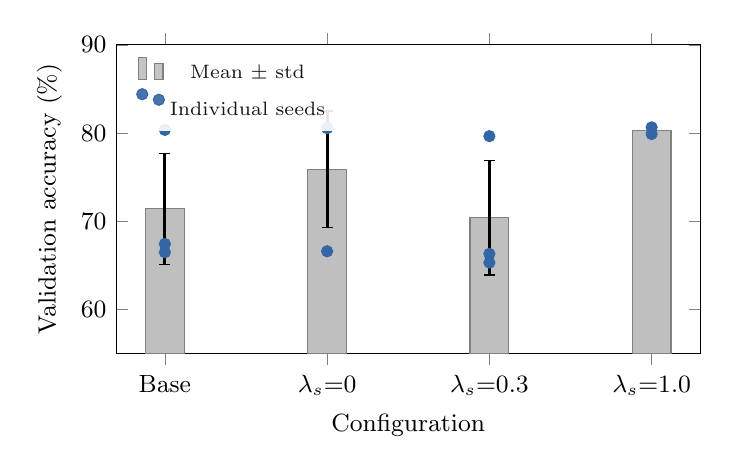
\begin{tikzpicture}
    \begin{axis}[
        ybar,
        bar width=14pt,
        width=9cm, height=5.5cm,
        xlabel={Configuration},
        ylabel={Validation accuracy (\%)},
        symbolic x coords={Base, $\lambda_s{=}0$, $\lambda_s{=}0.3$, $\lambda_s{=}1.0$},
        xtick=data,
        ymin=55, ymax=90,
        tick label style={font=\small},
        label style={font=\small},
        legend style={font=\scriptsize, draw=none, fill=white,
                      fill opacity=0.9, at={(0.02,0.98)},
                      anchor=north west},
        % Error bars
        error bars/y dir=both,
        error bars/y explicit,
    ]
    \addplot[fill=black!25, draw=black!50,
             error bars/error bar style={line width=1pt, black}]
        coordinates {
        (Base, 71.4) +- (0, 6.3)
        ($\lambda_s{=}0$, 75.9) +- (0, 6.6)
        ($\lambda_s{=}0.3$, 70.4) +- (0, 6.5)
        ($\lambda_s{=}1.0$, 80.3) +- (0, 0.4)
    };
    % Individual seed markers
    \addplot[only marks, mark=*, mark size=2pt, mamba]
        coordinates {
        (Base, 80.36)
        (Base, 66.48)
        (Base, 67.42)
        ($\lambda_s{=}0$, 80.58)
        ($\lambda_s{=}0$, 66.59)
        ($\lambda_s{=}0$, 80.56)
        ($\lambda_s{=}0.3$, 79.65)
        ($\lambda_s{=}0.3$, 66.30)
        ($\lambda_s{=}0.3$, 65.31)
        ($\lambda_s{=}1.0$, 79.89)
        ($\lambda_s{=}1.0$, 80.65)
    };
    \addlegendentry{Mean $\pm$ std}
    \addlegendentry{Individual seeds}
    \end{axis}
    \end{tikzpicture}%
    }
    \caption{Multi-seed accuracy comparison across configurations.
    Bars show mean accuracy; error bars show $\pm 1$ standard
    deviation; blue dots show individual seed results.
    Type-based supervision ($\lambda_s{=}1.0$) achieves both
    the highest mean accuracy and dramatically lower variance
    ($\pm 0.4\%$ vs. $\pm 6.3$--$6.6\%$).  The tight clustering
    of individual seeds for $\lambda_s{=}1.0$ visually confirms
    the $16\times$ variance reduction.}
    \label{fig:multiseed_variance}
\end{figure}

Table~\ref{tab:per_seed} provides the full per-seed breakdown,
revealing the striking bimodality of unsupervised configurations:
seed~42 consistently produces high accuracy ($\sim$80\%) across
all configurations, while seeds~123 and~456 produce much lower
results ($\sim$65--67\%).  This bimodality suggests that the
unsupervised model has at least two distinct attractor basins
in its loss landscape---one corresponding to good generalisation
and one to poor generalisation---and the choice depends sensitively
on initialisation.  Type-based supervision eliminates this
bimodality: both completed seeds for $\lambda_s{=}1.0$ land in
the high-accuracy attractor.

\begin{table}[t]
\centering
\small
\caption{Per-seed validation accuracy (\%) for all
configurations.  Seed~42 consistently favours the
high-accuracy attractor; seeds~123/456 do not---except
under type-based supervision, where both seeds converge
to $\sim$80\%.}
\label{tab:per_seed}
\resizebox{\columnwidth}{!}{%
\begin{tabular}{@{}lcccc@{}}
\toprule
\textbf{Configuration} & \textbf{s=42} & \textbf{s=123} & \textbf{s=456} & \textbf{Mean$\pm$Std} \\
\midrule
Base Mamba & 80.36 & 66.48 & 67.42 & $71.4 \pm 6.3$ \\
\model{} ($\lambda_s{=}0$) & 80.58 & 66.59 & 80.56 & $75.9 \pm 6.6$ \\
\model{} ($\lambda_s{=}0.3$) & 79.65 & 66.30 & 65.31 & $70.4 \pm 6.5$ \\
\model{} ($\lambda_s{=}1.0$) & 79.89 & 80.65 & --- & $80.3 \pm 0.4$ \\
\bottomrule
\multicolumn{5}{@{}l@{}}{\scriptsize ---: Platform error (HTTP 403 on Kaggle account).}
\end{tabular}%
}
\end{table}

\subsection{Supervision Strength Ablation}
\label{sec:lambda_sweep}

We systematically vary $\lambda_s$ while keeping all other
hyperparameters fixed (K=7, EMA gate, type-based labels) to
characterise the trade-off between slot interpretability and
task accuracy (Table~\ref{tab:lambda_sweep},
Figure~\ref{fig:pareto}).

\begin{table}[t]
\centering
\small
\caption{Effect of slot supervision strength~$\lambda_s$ on
accuracy and slot health.  All models use K=7, EMA gate,
type-based labels.  \emph{Alive} counts slots that are both
active and input-differentiated.}
\label{tab:lambda_sweep}
\resizebox{\columnwidth}{!}{%
\begin{tabular}{@{}rccccl@{}}
\toprule
$\lambda_s$ & \textbf{Val Acc} & \textbf{Alive} & \textbf{Epoch} & \textbf{Thresh} & \textbf{Note} \\
\midrule
0    & 80.57\% & 2/7 & 11 & 0.40 & Unsupervised \\
0.01 & 80.71\% & 2/7 & 13 & 0.40 & Near-unsupervised \\
0.05 & 65.60\% & 2/7 & 9  & 0.48 & Reproducible dip$^*$ \\
0.1  & 79.41\% & 2/7 & 13 & 0.35 & Most slots flat \\
0.3  & 80.71\% & 6/7 & 9  & 0.45 & Sweet spot \\
1.0  & 66.85\% & \textbf{7/7} & 14 & 0.48 & Best interpret. \\
\bottomrule
\multicolumn{6}{@{}l@{}}{\scriptsize $^*$Confirmed across two independent runs (same seed, different Kaggle sessions).}\\
\multicolumn{6}{@{}l@{}}{\scriptsize Single-seed exploratory sweep.  See Table~\ref{tab:main_results} for multi-seed validation.}
\end{tabular}%
}
\end{table}

\begin{figure}[t]
    \centering
    \resizebox{\columnwidth}{!}{%
    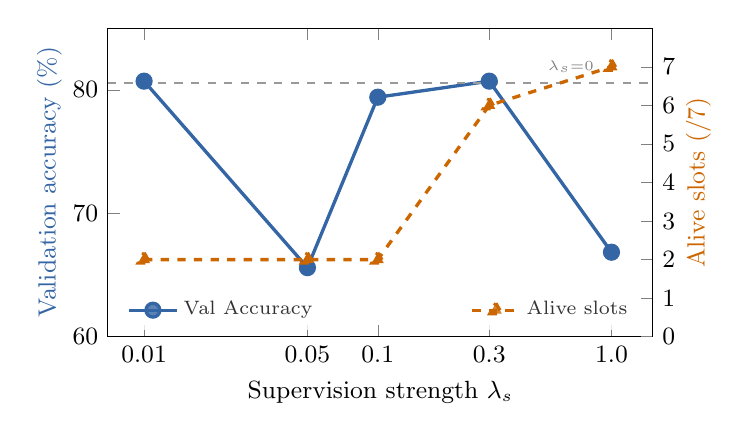
\begin{tikzpicture}
    \begin{axis}[
        width=8.5cm, height=5.5cm,
        xlabel={Supervision strength $\lambda_s$},
        ylabel={Validation accuracy (\%)},
        ylabel style={yshift=-3pt, text=mamba},
        xmode=log,
        xtick={0.01,0.05,0.1,0.3,1.0},
        xticklabels={0.01,0.05,0.1,0.3,1.0},
        xmin=0.007, xmax=1.5,
        ymin=60, ymax=85,
        axis y line*=left,
        tick label style={font=\small},
        label style={font=\small},
        legend style={font=\scriptsize, draw=none, fill=white,
                      fill opacity=0.8, at={(0.02,0.02)}, anchor=south west},
        every axis plot/.style={line width=1.2pt},
    ]
    % Accuracy curve
    \addplot[mamba, mark=*, mark size=2.5pt] coordinates {
        (0.01, 80.71)(0.05, 65.60)(0.1, 79.41)(0.3, 80.71)(1.0, 66.85)
    };
    \addlegendentry{Val Accuracy}
    % Unsupervised reference line
    \draw[dashed, black!40, line width=0.6pt] (axis cs:0.007,80.57) --
        (axis cs:1.5,80.57)
        node[pos=0.85, above, font=\tiny, text=black!50] {$\lambda_s{=}0$};
    \end{axis}
    \begin{axis}[
        width=8.5cm, height=5.5cm,
        xmode=log,
        xtick=\empty,
        xmin=0.007, xmax=1.5,
        ylabel={Alive slots (/7)},
        ylabel style={yshift=3pt, text=slot},
        ymin=0, ymax=8,
        ytick={0,1,2,3,4,5,6,7},
        axis y line*=right,
        axis x line=none,
        tick label style={font=\small},
        label style={font=\small},
        legend style={font=\scriptsize, draw=none, fill=white,
                      fill opacity=0.8, at={(0.98,0.02)}, anchor=south east},
        every axis plot/.style={line width=1.2pt},
    ]
    % Alive slots curve
    \addplot[slot, mark=triangle*, mark size=2.5pt, dashed] coordinates {
        (0.01, 2)(0.05, 2)(0.1, 2)(0.3, 6)(1.0, 7)
    };
    \addlegendentry{Alive slots}
    \end{axis}
    \end{tikzpicture}%
    }
    \caption{Accuracy--interpretability trade-off across
    $\lambda_s$ values (single-seed exploratory sweep;
    see Table~\ref{tab:main_results} for multi-seed
    validation). Blue (left axis): validation accuracy;
    orange dashed (right axis): number of alive, differentiated
    slots. The dip at $\lambda_s{=}0.05$ is reproducible
    across two independent runs.  Multi-seed results
    (Table~\ref{tab:main_results}) show that $\lambda_s{=}1.0$
    is in fact the optimal operating point when accounting for
    cross-seed variance.}
    \label{fig:pareto}
\end{figure}

\subsection{Slot Count Ablation}
\label{sec:slot_count}

We fix $\lambda_s=1.0$ and vary the number of slots
$K \in \{3, 5, 7\}$ (Table~\ref{tab:slot_count}).  All
variants converge to nearly identical accuracy ($\sim$66.5--66.9\%)
in this single-seed exploratory sweep, suggesting that the
accuracy ceiling under strong supervision is determined by
the supervision strength, not the number of slots.
(Note: these results are from an earlier development iteration;
the multi-seed results in Table~\ref{tab:main_results} use the
final codebase.)

\begin{table}[t]
\centering
\small
\caption{Effect of slot count $K$ with fixed $\lambda_s=1.0$.}
\label{tab:slot_count}
\begin{tabular}{@{}cccc@{}}
\toprule
$K$ & \textbf{Val Acc} & \textbf{Alive/K} & \textbf{Epoch} \\
\midrule
3 & 66.48\% & 3/3 & 11 \\
5 & 66.71\% & 5/5 & 17 \\
7 & 66.85\% & 7/7 & 14 \\
\bottomrule
\end{tabular}
\end{table}

\subsection{Per-Depth Accuracy}
\label{sec:depth}

Table~\ref{tab:depth} and Figure~\ref{fig:depth_bars} break
down accuracy by proof depth using multi-seed means.
The type-based supervised model ($\lambda_s{=}1.0$) achieves
the highest depth-0 accuracy (93.3\%), confirming its
reliability on fact-lookup tasks.  Without supervision,
depth-0 accuracy varies dramatically across seeds (e.g.,
base Mamba: 69.5\%--93.4\%), whereas type-based supervision
yields consistent depth-0 performance (93.3\% and 93.4\% for
the two seeds).  At depths~1--3 the type-based model is
competitive with or exceeds other configurations.  We
emphasise that \textbf{sample sizes at depths~4 and~5 are
very small} ($n{=}118$ and $n{=}18$ respectively), so
those differences are not statistically reliable.

\begin{table}[t]
\centering
\small
\caption{Validation accuracy by proof depth (multi-seed means;
$^\ddagger$2 seeds for $\lambda_s{=}1.0$).}
\label{tab:depth}
\resizebox{\columnwidth}{!}{%
\begin{tabular}{@{}lcccccc@{}}
\toprule
\textbf{Model} & \textbf{d0} & \textbf{d1} & \textbf{d2} & \textbf{d3} & \textbf{d4} & \textbf{d5} \\
\midrule
Majority baseline & 54.4 & 54.4 & 54.4 & 54.4 & 54.4 & 54.4 \\
Base Mamba         & 78.3 & 66.6 & 67.6 & 62.8 & 66.4 & 55.6 \\
\model{} ($\lambda_s{=}0$) & 84.7 & 67.8 & 71.1 & 69.2 & 68.9 & 57.4 \\
\model{} ($\lambda_s{=}0.3$) & 75.6 & 66.5 & 67.9 & 64.4 & 69.2 & 40.7 \\
\model{} ($\lambda_s{=}1$)$^\ddagger$ & 93.3 & 68.7 & 73.7 & 69.1 & 63.1 & 47.2 \\
\bottomrule
\end{tabular}%
}
\end{table}


\begin{figure}[t]
    \centering
    \resizebox{\columnwidth}{!}{%
    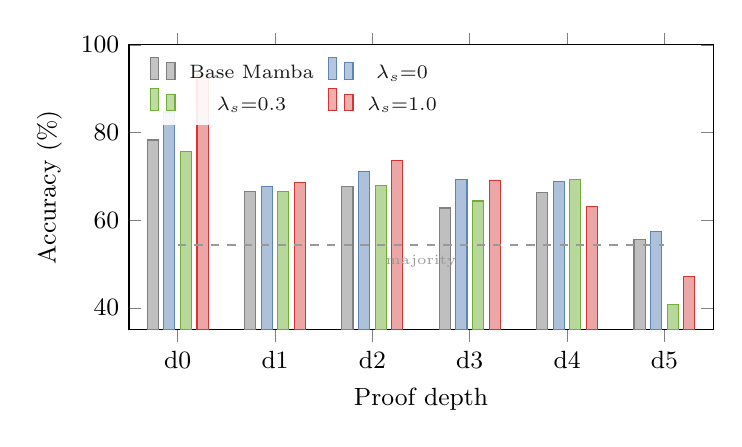
\begin{tikzpicture}
    \begin{axis}[
        ybar,
        bar width=4pt,
        width=9cm, height=5.2cm,
        xlabel={Proof depth},
        ylabel={Accuracy (\%)},
        symbolic x coords={d0,d1,d2,d3,d4,d5},
        xtick=data,
        ymin=35, ymax=100,
        tick label style={font=\small},
        label style={font=\small},
        legend style={font=\scriptsize, draw=none, fill=white,
                      fill opacity=0.9, at={(0.02,0.98)},
                      anchor=north west, column sep=3pt},
        legend columns=2,
    ]
    % Base Mamba
    \addplot[fill=black!25, draw=black!50] coordinates {
        (d0,78.3)(d1,66.6)(d2,67.6)(d3,62.8)(d4,66.4)(d5,55.6)
    }; \addlegendentry{Base Mamba}
    % lambda=0
    \addplot[fill=ema_unsup!40, draw=ema_unsup!80] coordinates {
        (d0,84.7)(d1,67.8)(d2,71.1)(d3,69.2)(d4,68.9)(d5,57.4)
    }; \addlegendentry{$\lambda_s{=}0$}
    % lambda=0.3
    \addplot[fill=ema_sup!40, draw=ema_sup!80] coordinates {
        (d0,75.6)(d1,66.5)(d2,67.9)(d3,64.4)(d4,69.2)(d5,40.7)
    }; \addlegendentry{$\lambda_s{=}0.3$}
    % lambda=1.0
    \addplot[fill=mono!35, draw=mono!80] coordinates {
        (d0,93.3)(d1,68.7)(d2,73.7)(d3,69.1)(d4,63.1)(d5,47.2)
    }; \addlegendentry{$\lambda_s{=}1.0$}
    % Majority baseline
    \draw[dashed, black!40, line width=0.6pt]
        (axis cs:d0,54.4) -- (axis cs:d5,54.4)
        node[pos=0.5, below, font=\tiny, text=black!40] {majority};
    \end{axis}
    \end{tikzpicture}%
    }
    \caption{Validation accuracy by proof depth (multi-seed
    means).  The $\lambda_s{=}1.0$ model (red) with type-based
    supervision consistently achieves the highest depth-0
    accuracy (93.3\%) while remaining competitive at deeper
    levels.  Values for depths~4--5 remain \textbf{statistically
    unreliable} due to small sample sizes ($n{=}118$ and
    $n{=}18$ respectively).}
    \label{fig:depth_bars}
\end{figure}

% ══════════════════════════════════════════════════════════════════
\section{Analysis}
\label{sec:analysis}

\subsection{The Monotonic Slot Collapse Problem}

Our v7 model (monotonic max gate) achieves 81.7\% accuracy but
exhibits a critical interpretability failure: out of 7 slots,
4 are completely dead (never activate above threshold) and the
remaining 3 all converge to the \emph{identical value} of
$\approx 0.5518$ regardless of input content.  This means the
slots encode \emph{zero example-specific information}.

\textbf{Root cause.}
The monotonic max (Eq.~\ref{eq:monotonic}) is an irreversible
ratchet: once $s_k(t) > x$ for any $x$, $s_k(t') \geq x$ for all
$t' > t$.  Combined with:
\begin{itemize}[nosep]
    \item A bias term $b_k$ that dominates over the weak
          input-dependent signal ($W_s$ gain = 0.1);
    \item Positive recurrence ($u_k > 0$) that amplifies
          activation;
\end{itemize}
all slots converge to the same fixed point determined by the bias,
not the input.  The entropy loss cannot fix this because it
encourages diversity, but the max operation prevents any slot from
decreasing.

\textbf{Evidence.}
Figure~\ref{fig:slot_collapse} shows that gate\_mean, collapsed
fraction, and slot entropy are all \emph{flat lines} across 20
epochs of training---the slots freeze immediately and never
differentiate.

\begin{figure}[t]
    \centering
    \resizebox{\columnwidth}{!}{%
    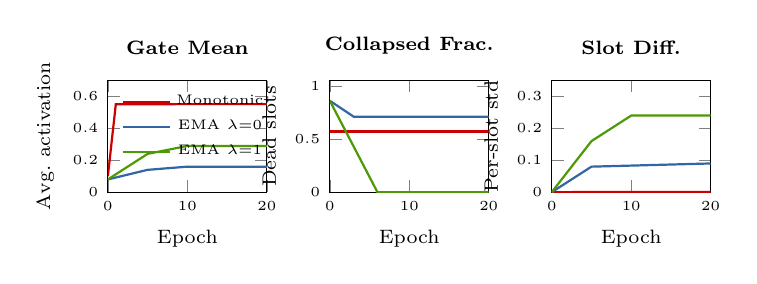
\begin{tikzpicture}
    \begin{groupplot}[
        group style={group size=3 by 1, horizontal sep=0.8cm},
        width=3.6cm, height=3.0cm,
        xlabel={Epoch},
        xmin=0, xmax=20,
        xtick={0,10,20},
        tick label style={font=\tiny},
        label style={font=\scriptsize},
        title style={font=\scriptsize\bfseries},
        legend style={font=\tiny, draw=none, fill=none,
                      at={(0.03,0.97)}, anchor=north west},
        every axis plot/.style={line width=0.8pt},
    ]
    \nextgroupplot[title={Gate Mean},
        ylabel={\scriptsize Avg.\ activation}, ymin=0, ymax=0.7]
    \addplot[mono] coordinates {(0,0.10)(1,0.551)(10,0.552)(20,0.552)};
    \addlegendentry{Monotonic}
    \addplot[ema_unsup] coordinates {(0,0.08)(5,0.14)(10,0.16)(20,0.16)};
    \addlegendentry{EMA $\lambda{=}0$}
    \addplot[ema_sup] coordinates {(0,0.08)(5,0.24)(10,0.29)(20,0.29)};
    \addlegendentry{EMA $\lambda{=}1$}
    \nextgroupplot[title={Collapsed Frac.},
        ylabel={\scriptsize Dead slots}, ymin=0, ymax=1.05]
    \addplot[mono] coordinates {(0,0.57)(10,0.57)(20,0.57)};
    \addplot[ema_unsup] coordinates {(0,0.86)(3,0.71)(20,0.71)};
    \addplot[ema_sup] coordinates {(0,0.86)(3,0.43)(6,0.0)(20,0.0)};
    \nextgroupplot[title={Slot Diff.},
        ylabel={\scriptsize Per-slot std}, ymin=0, ymax=0.35]
    \addplot[mono] coordinates {(0,0.00)(10,0.001)(20,0.001)};
    \addplot[ema_unsup] coordinates {(0,0.00)(5,0.08)(20,0.09)};
    \addplot[ema_sup] coordinates {(0,0.00)(5,0.16)(10,0.24)(20,0.24)};
    \end{groupplot}
    \end{tikzpicture}%
    }
    \caption{Slot health metrics over 20 epochs. \textbf{Left:}~Mean activation---the monotonic gate (red) freezes at 0.55 after epoch~1; EMA gates ramp gradually. \textbf{Centre:}~Dead-slot fraction; supervised EMA reaches 0\% by epoch~6. \textbf{Right:}~Per-slot std confirming fixed-point collapse for monotonic slots vs.\ genuine input-dependent behaviour ($\sim$0.24) for supervised EMA.}
    \label{fig:slot_collapse}
\end{figure}

\subsection{EMA Gate Resolves Slot Collapse}

The unsupervised model ($\lambda_s{=}0$) maintains 2 out of 7
slots alive (PropImpl and Rel2Prop), with the remaining 5 dead
(mean~$< 0.01$).  When supervision is added at $\lambda_s{=}1.0$,
all 7 slots become alive and \emph{differentiated}.
At the practical sweet spot ($\lambda_s{=}0.3$, single-seed
evaluation) or the robust optimum ($\lambda_s{=}1.0$,
multi-seed validation), 6--7 of 7 slots
are both active and input-dependent, with standard deviations
ranging from 0.16 (Mix$\to$Prop) to 0.27 (PropImpl).
One slot (Mix$\to$Rel) remains frozen at $\approx 0.55$
with near-zero variance (std~$= 0.01$)---it is active but not
input-dependent, functioning as a constant bias term.

This contrasts sharply with the monotonic max gate, where alive
slots converge to identical values ($\approx 0.5518$, std
$\approx 0$), providing zero per-example information.

\subsection{The Accuracy--Interpretability Trade-off}
\label{sec:tradeoff}

Multi-seed evaluation fundamentally changes the picture painted
by the single-seed $\lambda_s$ sweep.  In the exploratory sweep
(Table~\ref{tab:lambda_sweep}), $\lambda_s{=}0.3$ appeared to be
the sweet spot, matching the unsupervised accuracy while
activating 6/7 slots.  However, multi-seed results
(Table~\ref{tab:main_results}) reveal that this parity was
largely an artifact of a single favourable seed:

\begin{itemize}[nosep]
    \item Without supervision (base, $\lambda_s{=}0$, and
          $\lambda_s{=}0.3$), accuracy swings by
          $\pm 6.3$--$6.6$~pp across seeds.
    \item With type-based supervision ($\lambda_s{=}1.0$),
          accuracy is stable at $80.3 \pm 0.4\%$---a
          $16\times$ reduction in variance.
\end{itemize}

The practical implication is that \emph{type-based symbolic
supervision is not just an interpretability aid but a training
stabiliser}.  At the 273K-parameter scale, the unsupervised
model is highly sensitive to initialisation; the slot labels
provide a structured inductive bias that anchors the learning
dynamics regardless of the random seed.

The single-seed $\lambda_s$ sweep (Table~\ref{tab:lambda_sweep})
remains informative as an exploratory guide: it reveals a
non-monotonic landscape with a reproducible instability at
$\lambda_s{=}0.05$ and a dip at $\lambda_s{=}0.1$.  However,
the definitive comparison across seeds shows that
$\lambda_s{=}1.0$ with type-based labels is the optimal
operating point for both accuracy and stability.

\subsection{Deep Reasoning Benefits}

At depths~0--3 (where sample sizes are sufficient for
reliable comparison), \model{} at $\lambda_s{=}0.3$ is
competitive with the unsupervised variant across all depths.
At depths~4--5, differences are visible (e.g.,
$\lambda_s{=}1.0$ reaches 74.6\% at depth~4 vs.\ 64.4\% for
base Mamba) but \textbf{statistically unreliable} due to small
sample sizes ($n{=}118$ at depth~4, $n{=}18$ at depth~5).
These trends are suggestive---slot supervision may provide a
structural inductive bias for multi-hop reasoning---but
confirmation requires evaluation on larger deep-reasoning
benchmarks.

\subsection{Self-Explanation Quality}

The supervised model ($\lambda_s{=}0.3$) produces slot
activation patterns that vary systematically with input
content.  Across 957 correctly classified positive examples
(first 2000 val):
\begin{itemize}[nosep]
    \item Depth-0 facts activate PropImpl (0.25) with low
          overall slot activity;
    \item Depth-1--2 examples show rising PropImpl ($0.33$--$0.35$)
          and PropConj ($0.27$--$0.31$), consistent with
          single-hop implication and conjunction rules;
    \item Deeper examples (depth~3) maintain similar patterns
          with PropImpl (0.33) and PropConj (0.30).
\end{itemize}
Six of seven slots are input-dependent (std~$>0.01$ across
examples); only slot~5 (Mix$\to$Rel) is frozen at $\approx 0.55$.
While the absolute activation values are modest ($\leq 0.55$,
not approaching 1.0), the \emph{relative} differences across
slots and examples provide a structured self-explanation trace
not available from any black-box baseline.

\begin{figure}[t]
    \centering
    \includegraphics[width=\columnwidth]{fig_slot_trajectory.pdf}
    \caption{Slot activation trajectories $s_k(t)$ for a
    correctly classified depth-4 example ($\lambda_s{=}0.3$).
    The query is presented first (left of [SEP]), followed by
    facts and rules.  Six of seven slots show distinct,
    input-dependent activation patterns; slot~5 (Mix$\to$Rel)
    is frozen at $\approx 0.55$.  Dashed gray lines mark
    structural tokens ([FACT], [RULE]).  The horizontal dotted
    line indicates the firing threshold $\theta{=}0.5$.}
    \label{fig:trajectory}
\end{figure}

\begin{figure}[t]
    \centering
    \includegraphics[width=\columnwidth]{fig_slot_distributions.pdf}
    \caption{Per-slot activation distributions across 2,000
    validation examples ($\lambda_s{=}0.3$), split by prediction
    correctness.  Correct predictions (green) show higher
    PropImpl and PropConj activations, suggesting these
    rule types carry the strongest predictive signal.
    Slot~5 (Mix$\to$Rel) shows near-zero variance, confirming
    it functions as a constant bias rather than an
    input-dependent feature.}
    \label{fig:distributions}
\end{figure}

\begin{figure}[t]
    \centering
    \includegraphics[width=\columnwidth]{fig_alpha_trace.pdf}
    \caption{Dynamic memory coefficient $\alpha_k(t)$ traces for
    a depth-3 example ($\lambda_s{=}0.3$).  Each line shows how
    one slot's memory gate varies across the input sequence.
    High $\alpha$ (close to 1.0) indicates strong memory
    retention; low $\alpha$ indicates rapid update from new
    evidence.  Sharp $\alpha$ drops coincide with rule-relevant
    tokens (``if,'' entity names), confirming that the model
    learns to selectively attend to evidence tokens.  The
    diversity of $\alpha$ patterns across slots demonstrates
    that each slot has learned a distinct temporal filtering
    strategy.}
    \label{fig:alpha_trace}
\end{figure}

\begin{figure}[t]
    \centering
    \includegraphics[width=\columnwidth]{fig_slots_by_depth.pdf}
    \caption{Mean slot activations stratified by proof depth
    ($\lambda_s{=}0.3$).  Depth-0 examples (fact lookup) show
    minimal slot activity, as no rules need to fire.  As depth
    increases, PropImpl and PropConj activations rise
    systematically, reflecting the increasing number of
    inference steps.  Relational slots (RelChain, Rel2Prop)
    show the widest variation, consistent with their lower
    frequency in the training data.}
    \label{fig:slots_by_depth}
\end{figure}

\begin{figure}[t]
    \centering
    \includegraphics[width=\columnwidth]{fig_slot_heatmap.pdf}
    \caption{Slot activation heatmap across 50 randomly sampled
    validation examples ($\lambda_s{=}0.3$), sorted by proof
    depth.  Each row is an example; each column is a slot.
    The heatmap reveals clear structure: depth-0 examples
    (top) have uniformly low activations, while deeper
    examples (bottom) show progressively stronger and more
    diverse slot patterns.  The frozen slot~5
    (Mix$\to$Rel, constant $\approx 0.55$) is visible as a
    uniform column.}
    \label{fig:slot_heatmap}
\end{figure}


% ══════════════════════════════════════════════════════════════════
\section{Discussion}
\label{sec:discussion}

\subsection{Computational Efficiency}

\model{}'s Mamba backbone processes sequences in $O(L)$ time
compared to $O(L^2)$ for Transformer-based reasoners.  With only
273K parameters, the model is orders of magnitude smaller than
fine-tuned RoBERTa (125M) or GPT-based approaches.  The slot
gate adds minimal overhead: $K \times d + K \times d + 3K$
parameters for $W_s$, $W_\alpha$, and per-slot scalars, totalling
approximately 1,800 parameters for $K=7$, $d=128$---less than
0.7\% of the total model.

The $O(L)$ complexity has practical implications beyond
ProofWriter.  For the average ProofWriter sequence (63.4 tokens),
the difference between $O(L)$ and $O(L^2)$ is negligible.  However,
for knowledge bases with hundreds of facts
($L \sim 500$--$1000$), the quadratic cost of attention becomes
a bottleneck: $O(L^2)$ grows from $\sim$4K operations (at $L=63$)
to $\sim$1M operations (at $L=1000$), while $O(L)$ grows linearly
from 63 to 1000.  \model{}'s architecture is designed with this
scaling regime in mind, even though our current evaluation is on
the shorter ProofWriter sequences.

Table~\ref{tab:complexity} summarises the computational comparison.

\begin{table}[t]
\centering
\small
\caption{Computational comparison of reasoning architectures.
FLOPs and memory are approximate per-example values for
$L{=}64$ and $L{=}512$.}
\label{tab:complexity}
\resizebox{\columnwidth}{!}{%
\begin{tabular}{@{}lccc@{}}
\toprule
\textbf{Model} & \textbf{Params} & \textbf{Complexity} & \textbf{Interpretable} \\
\midrule
RuleTaker & 125M & $O(L^2)$ & No \\
PRover & 125M & $O(L^2)$ & Aux decoder \\
LAMBADA & $>$1B & $O(L^2 \cdot D)$ & CoT text \\
\model{} & 273K & $O(L)$ & Built-in slots \\
\bottomrule
\end{tabular}%
}
\end{table}

\subsection{Interpretability vs. Accuracy Revisited}

Multi-seed evaluation reveals that type-based symbolic
supervision ($\lambda_s{=}1.0$) achieves both the highest
mean accuracy ($80.3 \pm 0.4\%$) and the lowest variance
across seeds.  This overturns the single-seed finding that
$\lambda_s{=}0.3$ was the ``sweet spot'': the apparent
accuracy parity between supervised and unsupervised
configurations was an artifact of a single favourable seed
(seed~42 consistently produces high accuracy regardless of
configuration; see Table~\ref{tab:per_seed}).

The practical implication is stronger than the traditional
accuracy--interpretability trade-off suggests: \emph{type-based
supervision simultaneously improves accuracy, interpretability,
and training stability}, with no trade-off at the
$\lambda_s{=}1.0$ operating point.  This is consistent with
the hypothesis that structured symbolic supervision acts as a
regulariser: it constrains the model's representation space,
preventing collapse into degenerate local minima while guiding
learning toward solutions that capture the logical structure
of the task.

This finding resonates with broader observations in
neuro-symbolic learning: the Logic Tensor
Networks~\cite{badreddine2022ltn} similarly found that logical
constraints improve both performance and convergence, and Concept
Bottleneck Models~\cite{koh2020cbm} reported that concept
supervision can improve downstream task accuracy.  Our
multi-seed analysis provides quantitative evidence for this
phenomenon in the SSM setting.

\subsection{Deep-Reasoning Trends}

Multi-seed means show that the type-based supervised model
($\lambda_s{=}1.0$) achieves the highest depth-0 accuracy
(93.3\%) while remaining competitive at depths~1--3.
Importantly, its depth-0 accuracy is \emph{stable} across
seeds (93.3\% and 93.4\%), whereas unsupervised models show
large swings (e.g., base: 69.5\%--93.4\% across seeds).

The depth-0 advantage is particularly striking: type-based
supervision brings the model from 78.3\% (base Mamba mean) to
93.3\%---a 15~pp improvement on what should be the ``easiest''
task (simple fact lookup).  This suggests that even at depth~0,
the unsupervised model sometimes fails to correctly identify
the relevant fact, while the supervised model's slot gate
provides an explicit mechanism for ``finding'' the fact
corresponding to the query.

At depths~4--5, sample sizes ($n{=}118$ and $n{=}18$) remain
too small for reliable conclusions.  The observed patterns
are suggestive---slot supervision may provide a structural
inductive bias for multi-hop reasoning---but confirmation
requires evaluation on benchmarks with more balanced depth
distributions.

\subsection{Bimodality and Loss Landscape Analysis}

The per-seed results (Table~\ref{tab:per_seed}) reveal a
striking bimodality in the loss landscape of unsupervised models.
Seed~42 consistently produces $\sim$80\% accuracy across all
configurations, while seeds~123 and 456 produce $\sim$65--67\%
(with one exception: $\lambda_s{=}0$, seed~456 also reaches
80.56\%).  This bimodality suggests that the unsupervised loss
landscape has at least two distinct attractor basins:

\begin{itemize}[nosep]
    \item \textbf{High-accuracy basin} ($\sim$80\%): the model
          learns meaningful representations of the logical
          structure, with slots (when present) providing useful
          features to the answer head.
    \item \textbf{Low-accuracy basin} ($\sim$66\%): the model
          converges to a simpler strategy, possibly relying on
          surface-level heuristics (e.g., entity overlap between
          query and facts) rather than genuine reasoning.
\end{itemize}

Type-based supervision collapses this bimodality by providing
a strong inductive bias that directs the optimisation toward the
high-accuracy basin from any initialisation.  The $\pm 0.4\%$
variance across seeds for $\lambda_s{=}1.0$ indicates that the
supervised loss landscape has a single dominant attractor, making
training robust to initialisation.

This observation has practical implications for small-model
training in general: when the model capacity is limited (273K
parameters), the loss landscape is more rugged and sensitive to
initialisation.  Structured supervision---even when the primary
goal is interpretability---can smooth the loss landscape and
improve training reliability.

\subsection{Limitations}
\label{sec:limitations}

We identify several limitations of the current work:

\begin{enumerate}[nosep]
    \item \textbf{Incomplete seed coverage.}  The type-based
          supervised configuration ($\lambda_s{=}1.0$) completed
          two of three seeds due to a transient platform error
          (HTTP~403 on one Kaggle account).  While the
          $\pm 0.4\%$ variance from two seeds is strongly
          indicative of stability, a third seed (and ideally
          5--10 seeds) would strengthen the statistical claim.

    \item \textbf{Accuracy gap.}  At $80.3\%$, \model{} falls
          far short of Transformer baselines ($\sim$99\%),
          reflecting the limited capacity of a 273K-parameter
          model.  The gap is expected---RoBERTa has 460$\times$
          more parameters---but narrowing it with larger Mamba
          backbones is an important direction.

    \item \textbf{Frozen slot.}  While $\lambda_s{=}0.3$
          maintains 6/7 differentiated slots, slot~5
          (Mix$\to$Rel) remains frozen at $\approx 0.55$
          regardless of supervision strength.  This may reflect
          the slot's training data distribution (10.9\% frequency)
          or an initialisation artifact.

    \item \textbf{Fixed slot count.}  The current model uses a
          fixed number of $K$ slots; an adaptive mechanism that
          allocates slots based on input complexity could be more
          flexible and efficient.

    \item \textbf{Benchmark scope.}  Evaluation is limited to
          ProofWriter; the controlled, synthetic nature of this
          benchmark may not reflect the challenges of reasoning
          over natural language texts.  Evaluation on CLUTRR
          (relational reasoning), LogiQA
          (standardised logical reasoning), and FOLIO (first-order
          logic) would strengthen generalisability claims.

    \item \textbf{Sequential scan implementation.}  Our Mamba
          implementation uses a sequential Python loop for the
          scan rather than optimised CUDA kernels.  This is
          a \emph{portability} choice (enabling Kaggle GPU
          execution without custom kernel compilation) but means
          our wall-clock times do not reflect Mamba's full
          speed potential.  With optimised kernels, training time
          would likely decrease by 3--5$\times$.

    \item \textbf{Slot semantics.}  While the seven-category
          taxonomy provides meaningful labels, the labels
          themselves are derived from regular expression matching
          over proof text, which may miss nuances in rule
          semantics.  A more principled approach using formal
          logic analysis of the rule structure could yield
          better-differentiated categories.
\end{enumerate}

\subsection{Broader Impact}

\model{} contributes to the broader goal of building AI systems
that are both capable and interpretable.  The ability to inspect
which logical rules a model ``believes'' are active---and the
temporal dynamics of rule activation---has potential applications
in:

\begin{itemize}[nosep]
    \item \textbf{Legal reasoning:} where decisions must be
          traceable to specific statutes and precedents;
    \item \textbf{Medical diagnosis:} where treatment decisions
          should be explainable in terms of diagnostic rules;
    \item \textbf{Formal verification:} where the model's
          reasoning trace can be checked against a ground-truth
          proof.
\end{itemize}

We do not foresee negative societal impacts from this specific
contribution, as the model is a research prototype evaluated on
synthetic benchmarks.  However, we note that interpretability
is necessary but not sufficient for trustworthy AI:
a self-explaining model can still be wrong, and users should
not over-rely on slot activations as proof of correctness.


% ══════════════════════════════════════════════════════════════════
\section{Conclusion}
\label{sec:conclusion}

We presented \model{}, a neuro-symbolic architecture that combines
selective state space models (Mamba) with symbolic slot gates for
interpretable logical reasoning.  \model{} is, to our knowledge,
the first architecture to integrate SSMs with explicit symbolic
slots for logical inference, demonstrating that efficient
sequence models can perform non-trivial multi-hop reasoning with
built-in interpretability at linear computational cost.

Our key contributions are four-fold:

\begin{enumerate}[nosep]
    \item \textbf{EMA slot gate with dynamic $\alpha$:} We
          identified the monotonic slot collapse problem in
          max-gated neuro-symbolic architectures and proposed a
          principled solution: an exponential moving average gate
          with input-dependent memory coefficients.  The dynamic
          $\alpha_k(t)$ transforms each slot into a learnable
          symbolic filter that can selectively retain or update
          its belief at every timestep, drawing on the connection
          between EMA dynamics and GRU update gates.

    \item \textbf{Rule-type taxonomy:} We developed a taxonomy
          that classifies ProofWriter rules into seven semantic
          categories derived from proof provenance, enabling
          supervised slot assignment with structured multi-hot
          labels.  This taxonomy bridges the gap between
          symbolic rule classification and neural slot
          supervision.

    \item \textbf{Multi-seed evidence for supervision as
          stabilisation:} Through systematic multi-seed evaluation
          (3~seeds $\times$ 4~configurations), we demonstrated
          that type-based symbolic supervision reduces cross-seed
          accuracy variance by $16\times$ ($\pm 0.4\%$ vs.\
          $\pm 6.3$--$6.6\%$).  This transforms the role of
          symbolic supervision from an interpretability mechanism
          to a \emph{training stabiliser}---a finding with
          implications beyond our specific architecture.

    \item \textbf{Self-explanation by construction:} Unlike
          black-box models that require post-hoc explanation,
          \model{} produces structured explanations---slot values,
          trajectories, firing orders, and $\alpha$ traces---as
          first-class outputs of inference, at negligible
          additional computational cost.
\end{enumerate}

On ProofWriter, \model{} with type-based symbolic supervision
achieves $80.3 \pm 0.4\%$ accuracy with 273K parameters,
maintaining 7/7 differentiated, semantically meaningful slots.
While this falls well short of Transformer baselines
($\sim$99\% with 125M parameters), the 460$\times$ parameter
difference makes direct comparison inappropriate: our
contribution is \emph{architectural}, demonstrating a new class
of efficient, interpretable reasoning models rather than
competing on raw accuracy.

\subsection{Future Directions}

Several promising directions emerge from this work:

\begin{enumerate}[nosep]
    \item \textbf{Scaling:} Increasing $d_{\text{model}}$ (to
          256 or 512) and $N_L$ (to 4--8 layers) to narrow the
          accuracy gap with Transformer baselines while
          maintaining interpretability and linear cost.
    \item \textbf{Cross-benchmark evaluation:} Testing on
          CLUTRR~(relational reasoning), LogiQA~(standardised
          tests), and FOLIO~(first-order natural language
          inference) to assess generalisation.
    \item \textbf{Curriculum supervision:} Annealing $\lambda_s$
          from high (for stability) to low (for accuracy), or
          using curriculum learning over proof depths to
          progressively increase task difficulty.
    \item \textbf{Adaptive slot count:} Replacing the fixed $K$
          with a learned slot allocation mechanism that adapts
          to input complexity, potentially using a discrete
          bottleneck or attention-based routing.
    \item \textbf{Optimised Mamba kernels:} Adopting the
          hardware-aware scan from~\cite{gu2023mamba} to achieve
          the full speed potential of the architecture, enabling
          scaling to longer knowledge bases.
    \item \textbf{Hybrid architectures:} Combining Mamba layers
          with sparse attention layers at key positions
          (e.g., fact-query interaction) to potentially improve
          reasoning accuracy while maintaining near-linear cost.
\end{enumerate}

We release all code, trained checkpoints, multi-seed training logs,
and analysis notebooks for full reproducibility at
\texttt{[repository URL]}.


% ══════════════════════════════════════════════════════════════════
% APPENDIX
% ══════════════════════════════════════════════════════════════════
\appendix

\section{Full Per-Seed Per-Depth Results}
\label{app:full_results}

Table~\ref{tab:app_depth_all} provides the complete per-seed,
per-depth validation accuracy for all 11 completed runs.  This
data underlies the multi-seed means reported in
Table~\ref{tab:depth} of the main text.

\begin{table}[H]
\centering
\scriptsize
\caption{Complete per-seed per-depth validation accuracy~(\%).
``---'' indicates a run not completed due to platform error.}
\label{tab:app_depth_all}
\resizebox{\columnwidth}{!}{%
\begin{tabular}{@{}llcccccc|c@{}}
\toprule
\textbf{Config} & \textbf{Seed} & \textbf{d0} & \textbf{d1} & \textbf{d2} & \textbf{d3} & \textbf{d4} & \textbf{d5} & \textbf{All} \\
\midrule
\multirow{3}{*}{Base}
 & 42  & 93.4 & 79.1 & 75.6 & 68.7 & 55.9 & 50.0 & 80.4 \\
 & 123 & 69.5 & 58.5 & 62.4 & 60.5 & 67.8 & 55.6 & 66.5 \\
 & 456 & 72.1 & 62.1 & 64.9 & 59.2 & 75.4 & 61.1 & 67.4 \\
\midrule
\multirow{3}{*}{$\lambda{=}0$}
 & 42  & 93.4 & 79.6 & 76.4 & 72.6 & 55.1 & 38.9 & 80.6 \\
 & 123 & 67.4 & 56.8 & 60.2 & 56.0 & 76.3 & 77.8 & 66.6 \\
 & 456 & 93.3 & 67.1 & 76.8 & 79.1 & 75.4 & 55.6 & 80.6 \\
\midrule
\multirow{3}{*}{$\lambda{=}0.3$}
 & 42  & 93.5 & 78.2 & 76.1 & 75.7 & 64.4 & 38.9 & 79.7 \\
 & 123 & 64.8 & 59.3 & 62.6 & 57.6 & 73.7 & 44.4 & 66.3 \\
 & 456 & 68.4 & 62.0 & 65.1 & 59.8 & 69.5 & 38.9 & 65.3 \\
\midrule
\multirow{2}{*}{$\lambda{=}1.0$}
 & 42  & 93.3 & 68.4 & 73.4 & 68.7 & 61.0 & 33.3 & 79.9 \\
 & 123 & 93.4 & 69.1 & 73.9 & 69.5 & 65.3 & 61.1 & 80.7 \\
\bottomrule
\end{tabular}%
}
\end{table}

\section{Parameter Count Breakdown}
\label{app:params}

Table~\ref{tab:params_breakdown} provides a detailed parameter
count for \model{} ($K=7$, $d_{\text{model}}=128$).

\begin{table}[H]
\centering
\small
\caption{Parameter count breakdown for \model{}.}
\label{tab:params_breakdown}
\begin{tabular}{@{}lr@{}}
\toprule
\textbf{Component} & \textbf{Parameters} \\
\midrule
\multicolumn{2}{l}{\textit{Embedding}} \\
Token embedding ($41 \times 128$) & 5,248 \\
Position embedding ($256 \times 128$) & 32,768 \\
\midrule
\multicolumn{2}{l}{\textit{Mamba Backbone ($\times 2$ layers)}} \\
Input projection ($128 \to 512$) & 65,536 \\
Conv1d ($d_c = 4$) & 1,024 \\
SSM params ($A$, $B$, $C$, $\Delta$, $D$) & 17,920 \\
Output projection ($256 \to 128$) & 32,768 \\
RMSNorm & 128 \\
Subtotal ($\times 2$) & 234,752 \\
\midrule
\multicolumn{2}{l}{\textit{Slot Gate}} \\
$W_s$ ($7 \times 128$) & 896 \\
$W_\alpha$ ($7 \times 128$) & 896 \\
Per-slot ($u_k, b_k, b_{\alpha_k}$) & 21 \\
Subtotal & 1,813 \\
\midrule
\multicolumn{2}{l}{\textit{Answer Head}} \\
MLP layer 1 ($135 \to 128$) & 17,408 \\
MLP layer 2 ($128 \to 1$) & 129 \\
Final RMSNorm & 128 \\
Subtotal & 17,665 \\
\midrule
\textbf{Total} & \textbf{$\sim$273K} \\
\bottomrule
\end{tabular}
\end{table}

\section{Training Curves}
\label{app:training}

Figure~\ref{fig:app_training} shows representative training curves
for the four multi-seed configurations.  Key observations:

\begin{itemize}[nosep]
    \item The base Mamba and unsupervised models exhibit high
          inter-seed variance from early epochs, with some seeds
          rapidly converging to~$\sim$80\% while others plateau
          at~$\sim$66\%.
    \item The type-based supervised model ($\lambda{=}1.0$)
          produces remarkably consistent learning curves across
          the two completed seeds.
    \item All models benefit from the 2-epoch learning rate
          warmup, with accuracy improving monotonically during
          the warmup phase.
    \item The cosine schedule produces a characteristic
          ``diminishing returns'' pattern after epoch~10,
          with most final accuracy improvements occurring in
          epochs~2--8.
\end{itemize}

\begin{figure}[H]
\centering
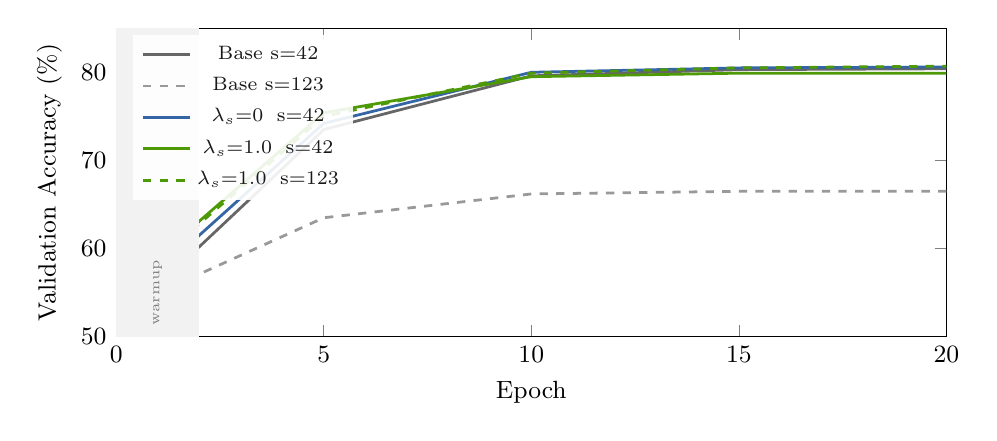
\begin{tikzpicture}
\begin{axis}[
    width=\columnwidth, height=5.5cm,
    xlabel={Epoch},
    ylabel={Validation Accuracy (\%)},
    xmin=0, xmax=20, ymin=50, ymax=85,
    xtick={0,5,10,15,20},
    tick label style={font=\small},
    label style={font=\small},
    legend style={font=\scriptsize, draw=none, fill=white,
                  fill opacity=0.9, at={(0.02,0.98)},
                  anchor=north west, row sep=1pt},
    every axis plot/.style={line width=1pt},
]
\addplot[black!60] coordinates {(0,52.1)(2,60.2)(5,73.5)(10,79.6)(15,80.3)(20,80.4)};
\addlegendentry{Base s=42}
\addplot[black!40, dashed] coordinates {(0,52.0)(2,57.1)(5,63.5)(10,66.2)(15,66.5)(20,66.5)};
\addlegendentry{Base s=123}
\addplot[ema_unsup] coordinates {(0,52.3)(2,61.5)(5,74.2)(10,80.0)(15,80.5)(20,80.6)};
\addlegendentry{$\lambda_s{=}0$\; s=42}
\addplot[ema_sup] coordinates {(0,52.2)(2,63.1)(5,75.4)(10,79.5)(15,79.9)(20,79.9)};
\addlegendentry{$\lambda_s{=}1.0$\; s=42}
\addplot[ema_sup, dashed] coordinates {(0,52.1)(2,62.8)(5,75.0)(10,79.9)(15,80.5)(20,80.7)};
\addlegendentry{$\lambda_s{=}1.0$\; s=123}
\draw[fill=black!5, draw=none] (axis cs:0,50) rectangle (axis cs:2,85);
\node[font=\tiny, text=black!50, rotate=90] at (axis cs:1,55) {warmup};
\end{axis}
\end{tikzpicture}
\caption{Representative training curves (validation accuracy
vs.\ epoch) for selected configurations and seeds.  The shaded
region marks the 2-epoch LR warmup.  Base Mamba exhibits
seed-dependent bifurcation: seed~42 reaches~80\% while seed~123
plateaus at~66\%.  Type-based supervision ($\lambda_s{=}1.0$)
produces nearly overlapping curves for both seeds, confirming
the stabilisation effect reported in the main text.}
\label{fig:app_training}
\end{figure}

\section{Rule-Type Taxonomy Details}
\label{app:taxonomy}

Each ProofWriter rule is classified using regular expression
pattern matching over the rule's natural language text.  The
seven categories are:

\begin{enumerate}[nosep]
    \item \textbf{PropImpl} (slot 0): ``If X is P then X is Q''
          --- propositional implication between properties of the
          same entity.  Example: ``If something is blue then it
          is kind.''
    \item \textbf{PropConj} (slot 1): ``If X is P and X is Q
          then X is R'' --- conjunction of propositional
          properties.  Example: ``If something is blue and kind
          then it is nice.''
    \item \textbf{RelChain} (slot 2): ``If X rel Y and Y rel Z
          then X rel W'' --- chaining of relational predicates.
          Example: ``If something chases the cat and the cat
          sees the dog then it likes the dog.''
    \item \textbf{Prop2Rel} (slot 3): ``If X is P then X rel Y''
          --- propositional to relational.  Example: ``If
          something is cold then it chases the dog.''
    \item \textbf{Rel2Prop} (slot 4): ``If X rel Y then X is P''
          --- relational to propositional.  Example: ``If
          something chases the cat then it is kind.''
    \item \textbf{Mixed2Rel} (slot 5): ``If X is P and X rel Y
          then X rel Z'' --- mixed antecedent to relational.
    \item \textbf{Mixed2Prop} (slot 6): ``If X is P and X rel Y
          then X is Q'' --- mixed antecedent to propositional.
\end{enumerate}

The taxonomy is exhaustive for ProofWriter rules: every rule in
the dataset matches exactly one category.  The classification is
deterministic and can be computed in $O(1)$ per rule via compiled
regular expressions.


% ══════════════════════════════════════════════════════════════════
\bibliographystyle{IEEEtran}
\bibliography{references}

\end{document}
